
\chapter*{Benchmarks and error framework}
\label{sec:org4e132ed}

In this chapter we describe the work developed during this study.
Since our main aim was to research on the mapping quality and the metrics used to assess it, we had to develop a whole framework in order to map and simulate quantum algorithm.
And, obviously, we had to have a set of quantum algorithms to map and simulate.

In the \hyperref[sec:orgbcda349]{Benchmarks} section we describe how we built the algorithm set.
In the \hyperref[sec:orgf9f9d14]{Error framework} section we describe the structure of the mapping of the algorithms procedure and its posterior metric calculation.
In order to use the mapping algorithm described in the \href{chapter-3.org}{Mapping model} section, we use OpenQL, a high level programming language to describe quantum circuits.
OpenQL is able to load a quantum device description and run our mapping algorithm, that is in its engine, to compile and export a mapped quantum circuit representation to the chosen device.
OpenQL will be explained in much detail in the section \hyperref[sec:org9083c76]{Compiler (OpenQL, cQASM)?}.

\section*{Benchmarks}
\label{sec:orgbcda349}
As stated in the Introduction, the research was conducted to analyze the different metrics to assert the quality of a mapping algorithm.
Consequently, we used a classic technique, the benchmarking technique.
In general computing, a benchmark is a program or a set of programs used to assess the performance of the host technology.
In our case, a benchmark would be a quantum algorithm that we will map to the SC chips constrains and then simulate aiming to use them to understand the different metrics.
Under this approach, it was decided that the best methodology would be to follow four steps.

\begin{enumerate}
\item Build algorithms list       
\begin{enumerate}
\item Gather the algorithms from \cite{zulehner17:effic_method_mappin_quant_circuit} and \cite{Lin_2014}.
\item Translate them from its QASM version to OpenQL.
\end{enumerate}
\item Algorithms profile (source, number of qubits, number of gates, gates percentage, \ldots{}).
\item Algorithms classification.
\item Mapping set creation
\end{enumerate}

\subsection*{Build a list of quantum algorithms}
\label{sec:orga3c88ab}

First, we built a list of quantum algorithms as benchmarks.
We opted to collect a big variety of different algorithms from different sources and libraries with a view to classify them and select the most interesting ones afterwards.
As it is common to find in the literature [REFER ALL THE PAPERS WITH LIST OF REAL BENCHMARKS], we also decided the benchmarks should be real and useful quantum algorithms, instead of random circuits.
The sources we chose are RevLib \cite{Wille_2008}, ScaffCC \cite{JavadiAbhari_2015}, some benchmarks from Zulehner's et al. work \cite{zulehner17:effic_method_mappin_quant_circuit} and QLib \cite{Lin_2014} because of the variety of algorithms and because they are decomposed in the Clifford+T set.
The counterpart is that the language description of the algorithms from those sources are different and any of them is the pure QASM, but OpenQASM or another altered QASM languages.
As mentioned in the introduction of this chapter and as it is shown in Section \hyperref[sec:org9083c76]{Compiler (OpenQL, cQASM)?}, in order to map the algorithms we will use the OpenQL tool.
Therefore we had to translate algorithms from their QASM versions to the OpenQL notation.
We developed a parser in python in order to do that.

\begin{table}[htbp]
\caption{\label{tab:orga0cc9ba}
Amount of algorithms per source organized per the type of circuit description language used}
\centering
\begin{tabular}{lrr}
\hline
OpenQASM & Altered QASM\\
\hline
RevLib () & QLib ()\\
ScaffCC () & \\
other Sources (1) & \\
\hline
\end{tabular}
\end{table}

\begin{figure}
\centering
\resizebox{0.75\textwidth}{!}{
\begin{tikzpicture}[>=stealth',shorten >=1pt,auto,node distance=0.7cm, thick,main node/.style={}]
    \fill[orange!40] (2,2) circle (.08cm) coordinate (Z);
    \fill[cyan!30] (3,6) circle (1.6cm) coordinate (R);
    \fill[purple!50] (7,5) circle (.1cm) coordinate (S);
    \fill[teal!40] (8,2) circle (1cm) coordinate (Q);
    \draw[gray,dashed] (5,4) ellipse (6cm and 4cm) coordinate (A);
    \draw (4,0) -- coordinate (L) (10,6.4) coordinate (Le);
 %\node[main node] (1) [left of R] {RevLib};
\node[main node] at (3,6) {RevLib};
\node[main node] (2) [above of=Z] {Others from Zulehner's paper};
\node[main node] (3) [above of=S] {ScaffCC};
%\node[main node] (4) [above right of Q] {QLib};
\node[main node] at (8,2) {QLib};
\node[main node,draw] (5) [above left  of=L] {OPENQASM};
\node[main node,draw] (6) [below of=Le] {QLib QASM};
\end{tikzpicture}
}
\label{fig:benchmarks_graph}
\caption{Graph depicting the amount of benchmarks per source. The line splits the source depending on the description programming language}
\end{figure}

\subsection*{Algorithms profile}
\label{sec:orgdb2051f}

The goal of this second step is to understand the algorithms we have, extracting their statistics.
We built a benchmark profile with the number of qubits used, the number of gates, the expected behaviour of the algorithm and different graphs, showing the percentage of the operations types or the number of operations running in parallel amongst others.

\subsection*{Benchmarks classification}
\label{sec:org2731fa8}

The third step is to classify the benchmarks depending on their behaviour.
This is an important step because algorithms that do similar calculations are used to have common gates distribution.
From all the benchmarks we have, we can distinct six different classes.

\begin{itemize}
\item Quantum Gates: Circuits that are a decomposition of a Quantum Gate
\item Search Algorithms
\item Worst Cases: Circuits that were really difficult to generate for RevLib
\begin{itemize}
\item HWB: is the simplest function with exponential Ordered Binary Decision Diagrams (OBDD) size.
\end{itemize}
\item Encoding Functions: Classical codification functions
\item Arithmetic Functions: Functions that perform an arithmetic operation
\item Miscellaneous: Mix of different kind of algorithms that we do not know its expected behavior
\end{itemize}


\subsection*{Benchmarks selection}
\label{sec:org4ddbf91}

The last step aims to have a small, but representative, set of benchmarks to map.
This requirement comes by the fact that simulations are long and computationally exhaustive.
In order to do that, we studied the different benchmark profiles looking for most illustrative cases.
But we also set some restrictions.
First of all, as soon as we are going to map the algorithms to the SC chips with a maximum number of 17 qubits, we need to look for the benchmarks with an amount of qubits below that.
We also want to see how different gate quantities affect the mapping.
Therefore, we need benchmarks with a number of gates as spread as possible.
And, at the same time, several benchmarks presenting the same number of gates.
We also tend to mix all the classes equally.
And we try to have the less number of the same algorithm versions as possible.
We only take the same algorithm versions for cases in which the number of qubits and the number of gates show an interesting combination.
For example, two similar algorithms which number of qubits or number of gates are very distinct as the first three selected benchmarks in Tab. \ref{tab:orgc368478}.
Finally, benchmarks with a known functionality are preferred.

Once we had our requirements we could start the analysis and the selection afterwards.
In the next figures, from Fig. \ref{code:no_q_statistics} to Fig. \ref{code:q_gate_bench}, we show the different steps and data of the analysis in order to do the selection.
In Tab. \ref{tab:orgc368478} we show the final benchmark selection.
The crossed out algorithms are the ones that, after the selection, the simulation failed because of their computational requirements.
\begin{table}[htbp]
\caption{\label{tab:org86eed0e}
Restriction summary of the benchmark selection}
\centering
\begin{tabular}{|l|}
\hline
\\
Restrictions:\\
\\
- \# qubits < 17\\
- \# gates as spread as possible and in the case of repeated benchmark the minimum number of gates\\
- The less number of the same algorithm versions/classes as possible\\
- The benchmarks that are repeated and have an interesting combination of No. qubits/No. gates are  preferred\\
- The benchmarks with a known functionality are preferred\\
\\
\hline
\end{tabular}
\end{table}

\begin{figure}
\centering

\begin{verbatim}

            Benchmarks ammount
No. qubits
3                           12
4                           12
5                           57
6                           31
7                           22
8                           16
9                           15
10                          21
11                          17
12                          14
13                          18
14                          17
15                          16
16                          14
17                          10

\end{verbatim}


\label{code:no_q_statistics}
\caption{Statistics of the amount of benchmarks wit the same number of qubits}
\end{figure}
[TOPLOT]

\begin{verbatim}

[4, 5, 6, 7, 8, 9, 10, 11, 12, 13, 14, 15, 16, 17, 18, 19, 20, 21, 22, 23, 25, 27, 28, 29, 31, 33, 34, 35, 36, 37, 43, 50, 51, 52, 53, 66, 68, 69, 70, 73, 83, 84, 85, 91, 103, 107, 110, 115, 131, 132, 146, 148, 150, 151, 162, 163, 164, 173, 175, 178, 179, 194, 200, 211, 215, 217, 228, 230, 231, 233, 235, 244, 247, 251, 258, 263, 270, 272, 273, 275, 288, 290, 296, 320, 326, 328, 338, 342, 343, 395, 403, 440, 451, 467, 469, 485, 504, 555, 580, 612, 631, 650, 778, 781, 954, 986, 1043, 1206, 1221, 1291, 1336, 1776, 1914, 1993, 3009, 3073, 3213, 3439, 3888, 4813, 5321, 6050, 6723, 7630, 8763, 9462, 10223, 10619, 11414, 13658, 17159, 17936, 18852, 20112, 21504, 22445, 24379, 27126, 33827, 34881, 38046, 38577, 49829, 54766, 64283, 69380, 80480, 125362, 128744, 164416, 171840, 184864, 187112, 207775, 360618, 423488, 512064]

\end{verbatim}

\begin{figure}
\centering

\begin{verbatim}

                      Benchmarks ammount
No. qubits No. gates
3          6                           7
           7                           1
           19                          1
           20                          1
           36                          1
           50                          1
4          8                           6
           9                           2
           34                          1
           36                          1
           51                          1
           52                          1
5          4                           1
           7                           1
           10                          5
           11                          3
           18                          1
           20                          1
           21                          1
           22                          1
           23                          1
           27                          1
           35                          2
           36                          2
           37                          5
           52                          1
           53                          1
           66                          1
           68                          1
           69                          3
...                                  ...
13         128744                      1
           360618                      1
14         28                          1
           29                          8
           211                         1
           270                         1
           1776                        2
           11414                       1
           33827                       1
           38577                       1
           187112                      1
15         31                          8
           37                          1
           343                         1
           4813                        1
           7630                        1
           8763                        1
           9462                        1
           17936                       1
           171840                      1
16         33                          8
           175                         1
           272                         1
           326                         1
           485                         1
           10619                       1
           18852                       1
17         35                          8
           36                          1
           43                          1

[180 rows x 1 columns]

\end{verbatim}



\label{code:q_gate_bench}
\caption{Amount of benchmarks classified by the number of gates and the number of qubits}
\end{figure}
43 benchmarks (with qubits numbers from 3 to 17 qubits) selected after applying the previous Restrictions to the analysis of the benchmarks described in the next section.

After simulating the algorithms, some of them either return errors (segmentation fault) or are computationally exhausting to simulate them as they should be simulated.

\begin{table}[htbp]
\caption{\label{tab:orgc368478}
Table of the selected benchmarks to be mapped. Note that the crossed ones mean that they were to computationally exhaustive and the simulations failed.}
\centering
\begin{tabular}{lll}
\hline
No. qubits & No. gates & Algorithm\\
\hline
5 & 27 & \texttt{4gt11\_82}\\
6 & 228 & \texttt{4gt12-v1\_89}\\
6 & 258 & \texttt{4gt4-v0\_72}\\
7 & 70 & \texttt{4mod5-bdd\_287}\\
5 & 20 & \texttt{4mod5-v0\_20}\\
7 & 84 & \texttt{alu-bdd\_288}\\
5 & 36 & \texttt{alu-v0\_27}\\
17 & 35 & \texttt{benstein\_vazirani\_15b\_secret\_128}\\
16 & 175 & \texttt{+cnt3-5\_179+}\\
5 & 7 & \texttt{cuccaroAdder\_1b}\\
7 & 11 & \texttt{cuccaroMultiplier\_1b}\\
6 & 73 & \texttt{decod24-bdd\_294}\\
6 & 338 & \texttt{decod24-enable\_126}\\
6 & 5 & \texttt{graycode6\_47}\\
13 & 360618 & \texttt{+ground\_state\_estimation\_10+}\\
3 & 16 & \texttt{grover\_orcl\_toff}\\
3 & 20 & \texttt{ham3\_102}\\
5 & 233 & \texttt{hwb4\_49}\\
10 & 200 & \texttt{+ising\_model\_10+}\\
11 & 22445 & \texttt{+life\_238+}\\
3 & 50 & \texttt{miller\_11}\\
5 & 288 & \texttt{mini-alu\_167}\\
10 & 173 & \texttt{+mini\_alu\_305+}\\
5 & 178 & \texttt{mod10\_176}\\
6 & 555 & \texttt{mod5adder\_127}\\
5 & 22 & \texttt{mod5d1\_63}\\
6 & 440 & \texttt{mod8-10\_177}\\
5 & 132 & \texttt{one-two-three-v1\_99}\\
5 & 70 & \texttt{one-two-three-v3\_101}\\
13 & 128744 & \texttt{+plus63mod4096\_163+}\\
10 & 110 & \texttt{+qft\_10+}\\
4 & 34 & \texttt{rd32-v0\_66}\\
6 & 781 & \texttt{sf\_274}\\
6 & 778 & \texttt{sf\_276}\\
12 & 4792 & \texttt{shor\_15}\\
12 & 3009 & \texttt{sqrt8\_260}\\
13 & 1993 & \texttt{+squar5\_261+}\\
15 & 7630 & \texttt{+square\_root\_7+}\\
7 & 3888 & \texttt{sym6\_145}\\
14 & 270 & \texttt{+sym6\_316+}\\
8 & 80480 & \texttt{+urf2\_152+}\\
8 & 20112 & \texttt{+urf2\_277+}\\
8 & 12 & \texttt{vbeAdder\_2b}\\
6 & 7 & \texttt{xor5\_254}\\
\hline
\end{tabular}
\end{table}



\subsection*{Github repository}
\label{sec:org268cb6d}

Finally, all this information is detailed in the \href{https://github.com/QE-Lab/qbench}{qbench Github repo} where one can find all the benchmarks, as well.

\section*{Error framework}
\label{sec:orgf9f9d14}
In this section we introduce the framework we developed in order to analyze the quantum metrics.

\subsection*{Compiler (OpenQL, cQASM)?}
\label{sec:org9083c76}
[Intro]


\begin{figure}[htbp]
\centering
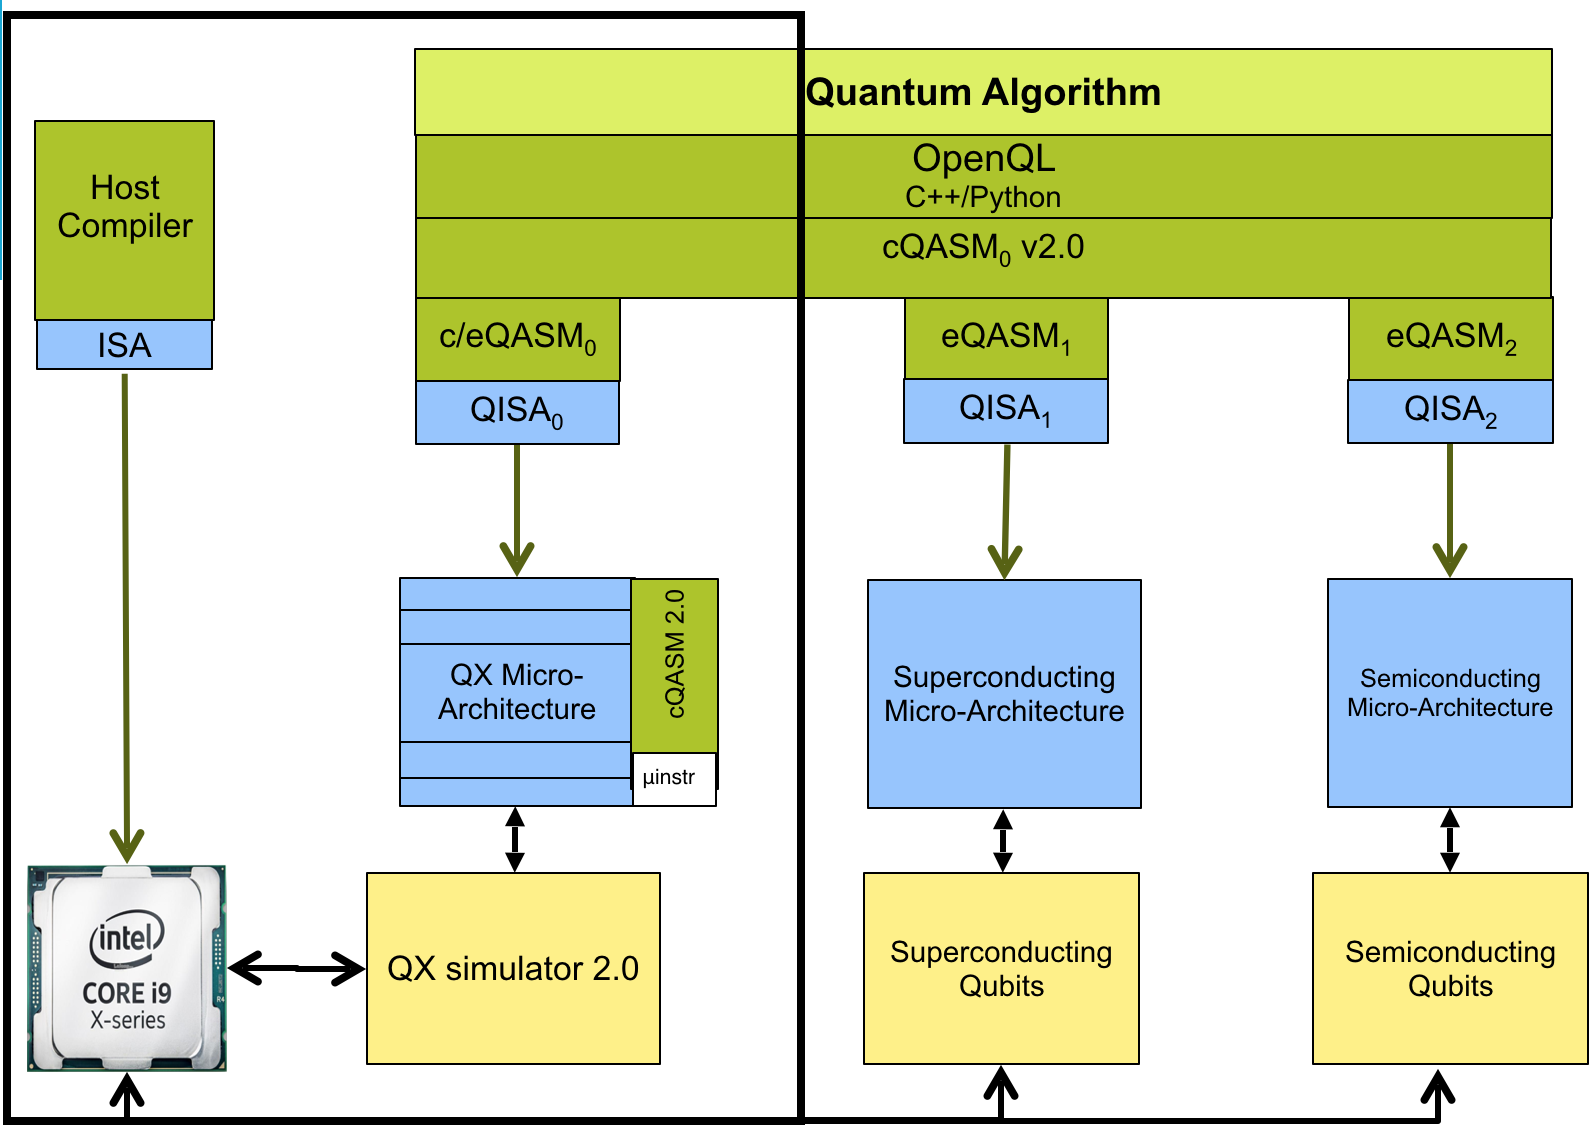
\includegraphics[width=\textwidth]{figures/layers.png}
\caption{\label{fig:orgda7e1c5}
Compilation layers}
\end{figure}


\begin{itemize}
\item cQASM
\label{sec:org5361516}


\item OpenQL
\label{sec:orgef7eeea}

\begin{figure}[htbp]
\centering
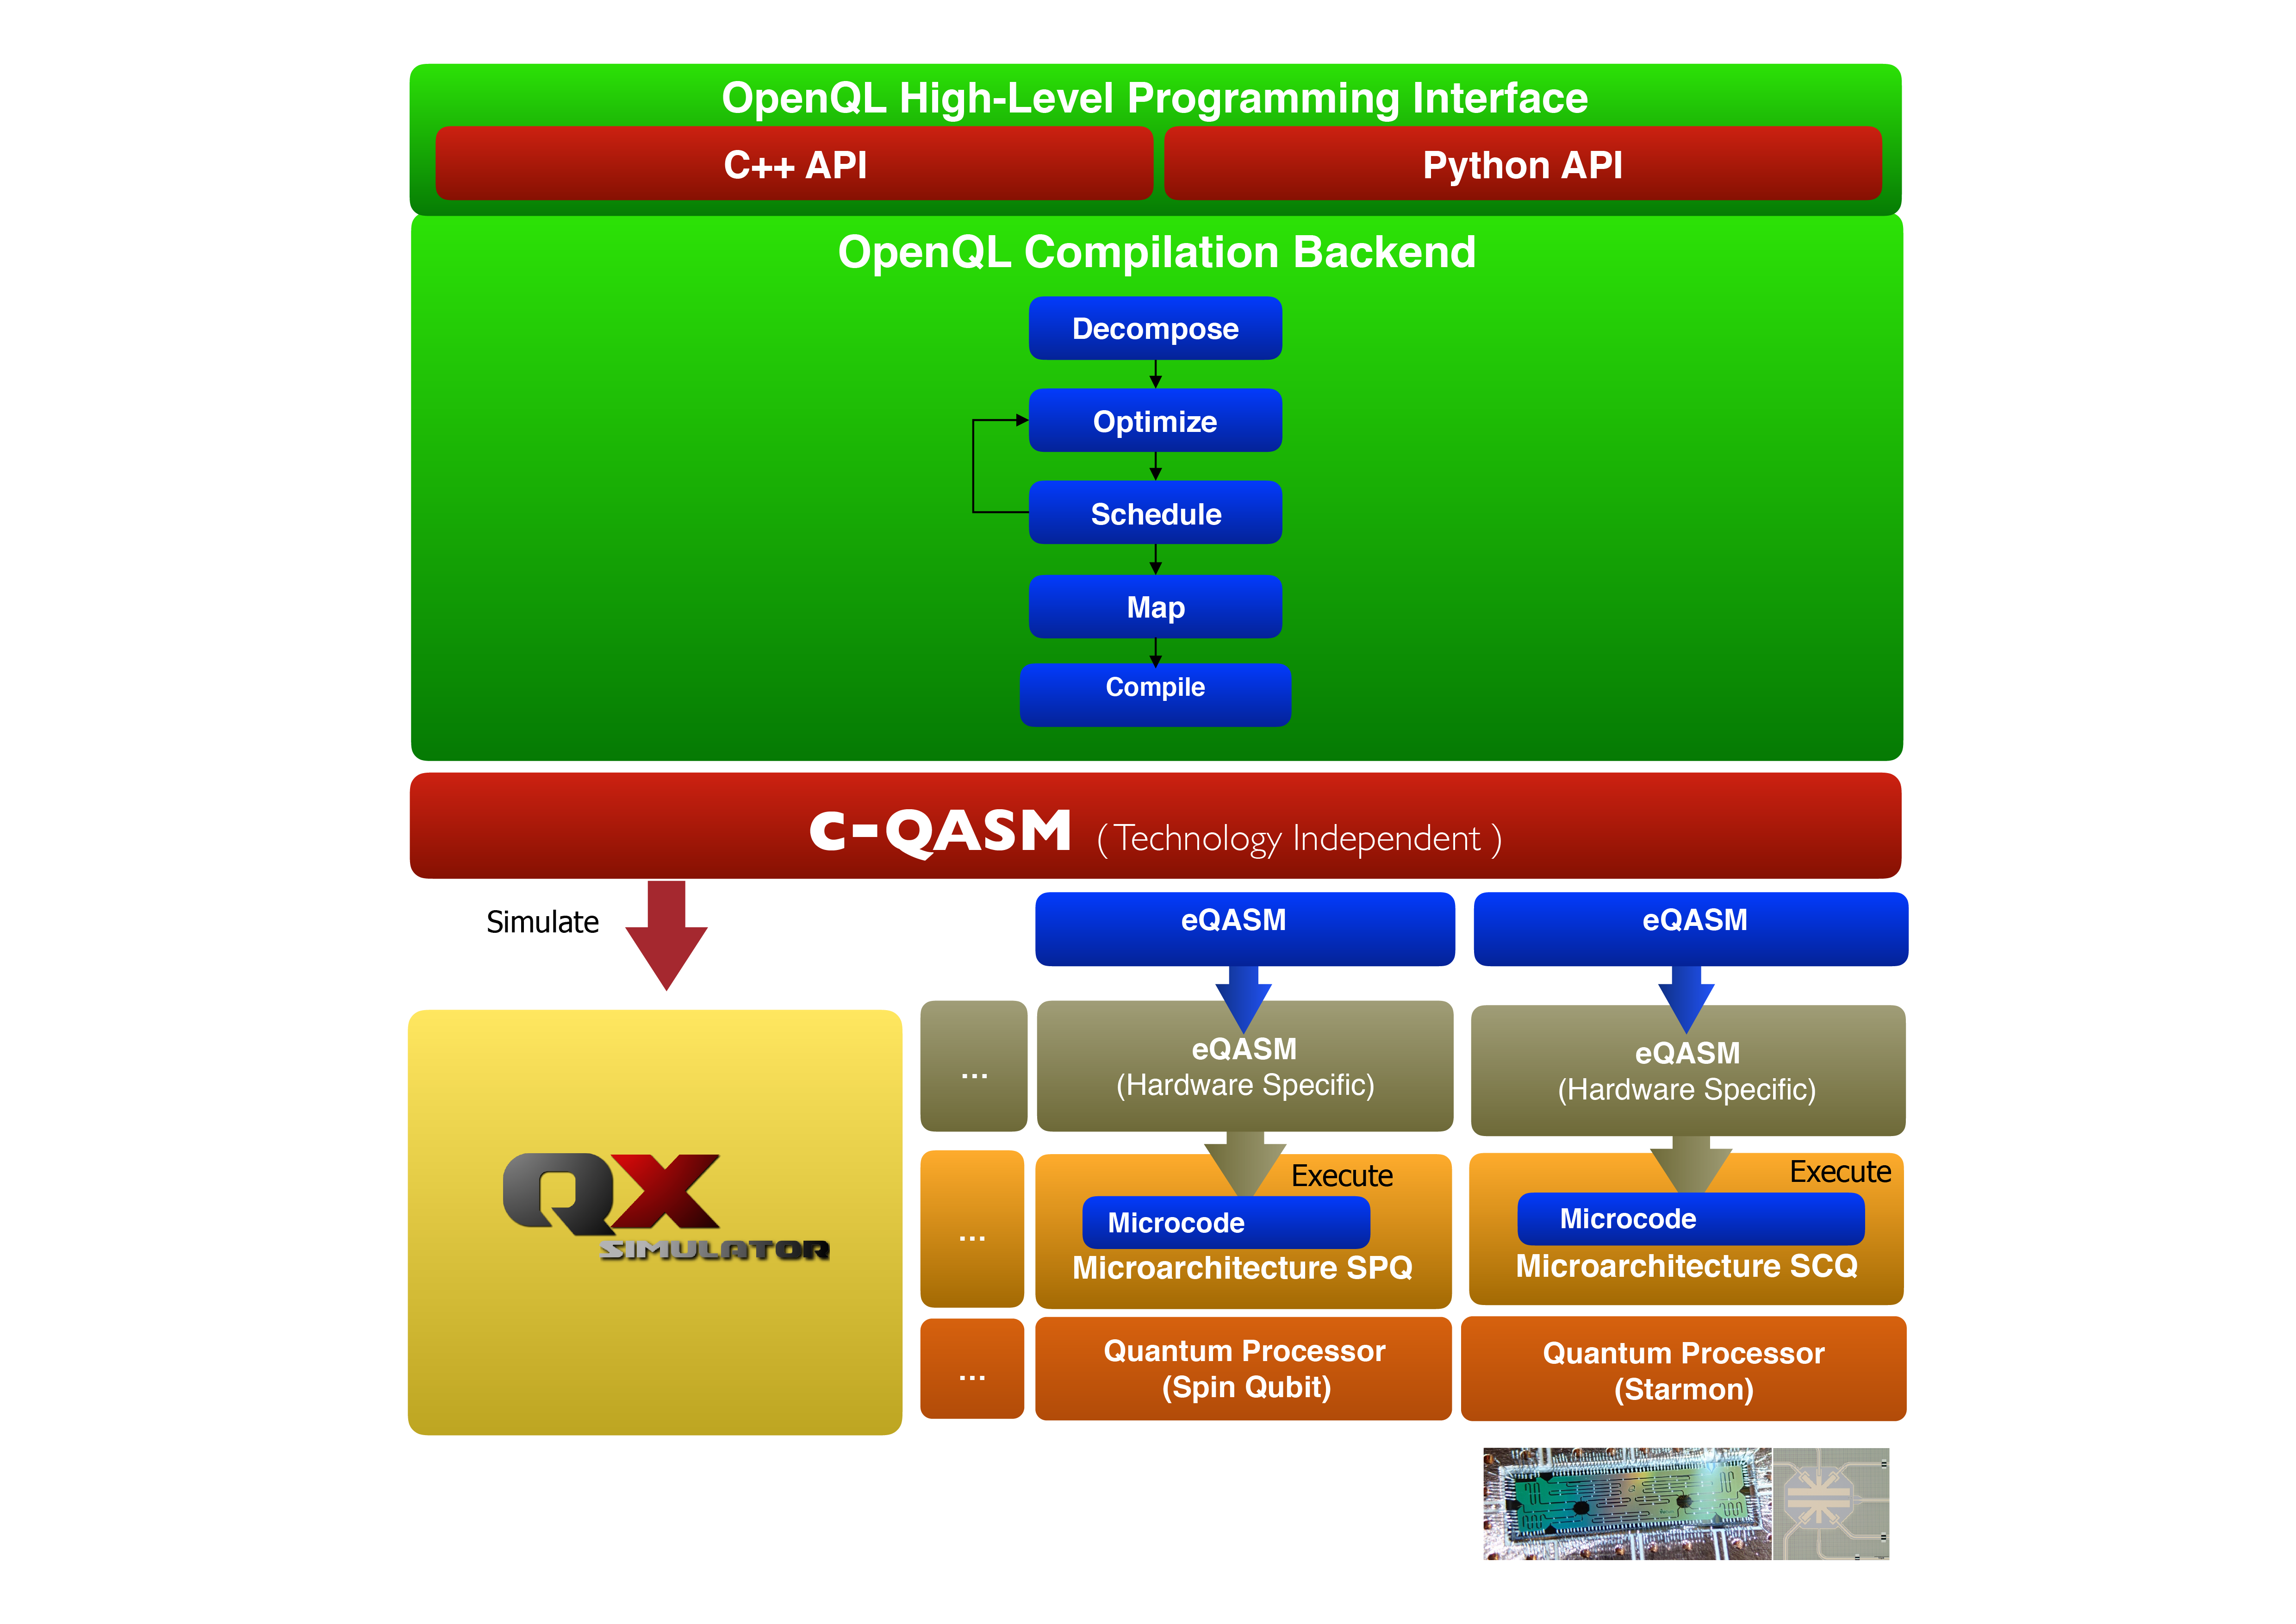
\includegraphics[width=0.9\textwidth]{figures/openql.png}
\caption{\label{fig:org8ef65be}
OpenQL diagram}
\end{figure}

\begin{figure}
\centering
\begin{minipage}{\textwidth}

\begin{minted}[frame=lines,fontsize=\scriptsize,linenos,breaklines,breakanywhere]{python}

from openql import openql as ql
import os
import argparse

def circuit(config_file, scheduler='ASAP', uniform_sched= 'no', mapper='base', initial_placement='no', output_dir_name='test_output', optimize='no', measurement=True, log_level='LOG_WARNING'):
    curdir = os.path.dirname(__file__)
    output_dir = os.path.join(curdir, output_dir_name)
    ql.set_option('output_dir', output_dir)
    ql.set_option('optimize', optimize)
    ql.set_option('scheduler', scheduler)
    ql.set_option('scheduler_uniform', uniform_sched)
    ql.set_option('mapper', mapper)
    ql.set_option('initialplace', initial_placement)
    ql.set_option('log_level', log_level)

    config_fn = os.path.join(curdir, config_file)

    platform  = ql.Platform('starmon', config_fn)
    sweep_points = [1,2]
    num_circuits = 1
    num_qubits = 6
    p = ql.Program('graycode6', platform, num_qubits)
    p.set_sweep_points(sweep_points, num_circuits)
    k = ql.Kernel('graycode6', platform, num_qubits)
    k.gate('cnot',[1,0])
    k.gate('cnot',[2,1])
    k.gate('cnot',[3,2])
    k.gate('cnot',[4,3])
    k.gate('cnot',[5,4])

    if measurement:
	for q in range(num_qubits):
	    k.gate('measure', [q])

    p.add_kernel(k)
    p.compile()

\end{minted}

\caption{OpenQL description in python code describing the Gray code algorithm.}
\label{code:openql_gray_code}
\end{minipage}
\end{figure}

\begin{figure}
\centering
\begin{minipage}{\textwidth}

\begin{minted}[frame=lines,fontsize=\scriptsize,linenos,breaklines,breakanywhere]{js}

{
   "eqasm_compiler" : "cc_light_compiler",

   "hardware_settings": {
	 "qubit_number": 7,
	 "cycle_time" : 20,  
     ...
   },

  "resources":
   {
    "qubits":
    {
      "description": "Each qubit can be used by only one gate at a time. There are 'count' qubits.",
      "count": 7
    },
    "qwgs" :
    {
      "description": "Single-qubit rotation gates (instructions of 'mw' type) are controlled by qwgs.  Each qwg controls a private set of qubits.  A qwg can control multiple qubits at the same time, but only when they perform the same gate and started at the same time. There are 'count' qwgs. For each qwg it is described which set of qubits it controls.",
      "count": 3,
      "connection_map":
      {
	"0" : [0, 1],
	"1" : [2, 3, 4],
	"2" : [5, 6]
      }
    },
    "meas_units" :
    {
      "description": "Single-qubit measurements (instructions of 'readout' type) are controlled by measurement units.  Each one controls a private set of qubits.  A measurement unit can control multiple qubits at the same time, but only when they started at the same time. There are 'count' measurement units. For each measurement unit it is described which set of qubits it controls.",
      "count": 2,
      "connection_map":
      {
	"0" : [0, 2, 3, 5, 6],
	"1" : [1, 4]
      }
    },
    "edges":
    {
      "description": "Two-qubit flux gates (instructions of 'flux' type) are controlled by qubit-selective frequency detuning.  Frequency-detuning may cause neighbor qubits (qubits connected by an edge) to inadvertently engage in a two-qubit flux gate as well. This happens when two connected qubits are both executing a two-qubit flux gate. Therefore, for each edge executing a two-qubit gate, certain other edges should not execute a two-qubit gate. There are 'count' edges. For each edge it is described which set of other edges cannot execute a two-qubit gate in parallel.",
      "count": 16,
      "connection_map":
      {
	"0": [2, 10], 
	...
	"15": [5, 13]
      }
    },
    "detuned_qubits":
    {
      "description": "A two-qubit flux gate lowers the frequency of its source qubit to get near the frequency of its target qubit.  Any two qubits which have near frequencies execute a two-qubit flux gate.  To prevent any neighbor qubit of the source qubit that has the same frequency as the target qubit to interact as well, those neighbors must have their frequency detuned (lowered out of the way).  A detuned qubit cannot execute a single-qubit rotation (an instruction of 'mw' type).  An edge is a pair of qubits which can execute a two-qubit flux gate.  There are 'count' qubits. For each edge it is described, when executing a two-qubit gate for it, which set of qubits it detunes.",
      "count": 7,
      "connection_map":
      {
	"0": [3],
	...
	"15": []
      }
    }
  },
  "topology" : 
  {
    "description": "A qubit grid is rectangular. The coordinates in the X direction are 0 to x_size-1. In the Y direction they are 0 to y_size-1. In the grid real qubits are placed. Each qubit has an id (its index, used above in the resource descriptions, and used below as operands to gates), an x and a y coordinate. Qubits are connected in directed pairs, called edges. Each edge has an id (its index, used above in the resource descriptions), a source qubit and a destination qubit.",
    "x_size": 5,
    "y_size": 3,
    "qubits": 
    [ 
      { "id": 0,  "x": 1, "y": 2 },
      ...
      { "id": 6,  "x": 3, "y": 0 }
    ],
    "edges": 
    [
      { "id": 0,  "src": 2, "dst": 0 },
      ...
      { "id": 15,  "src": 4, "dst": 6 }

    ]
  },

   "instructions": {

   "measure": {
      "duration": 320,
      "latency": 0,
      "matrix": [ [0.0,1.0], [1.0,0.0], [1.0,0.0], [0.0,0.0] ],
      "disable_optimization": false,
      "type": "readout",
      "cc_light_instr_type": "single_qubit_gate",
      "cc_light_instr": "measz",
      "cc_light_opcode": 4
   },
   "i": {
      "duration": 20,
      "latency": 0,
      "matrix": [ [0.0,1.0], [1.0,0.0], [1.0,0.0], [0.0,0.0] ],
      "disable_optimization": false,
      "type": "mw",
      "cc_light_instr_type": "single_qubit_gate",
      "cc_light_instr": "i",
      "cc_light_opcode": 5
   },
   "x": {
      "duration": 20,
      "latency": 0,
      "matrix": [ [0.0,1.0], [1.0,0.0], [1.0,0.0], [0.0,0.0] ],
      "disable_optimization": false,
      "type": "mw",
      "cc_light_instr_type": "single_qubit_gate",
      "cc_light_instr": "x",
      "cc_light_opcode": 6
   }

   ...

   },

    "gate_decomposition": {
	"cnot %0 %1": ["ym90 %1","cz %0 %1","ry90 %1"],
	"swap %0 %1": ["ym90 %1","cz %0 %1","ry90 %1", "ym90 %0","cz %1 %0","ry90 %0", "ym90 %1","cz %0 %1","ry90 %1"],
	"z %0" : ["x %0","y %0"],
    ...
    }
}


\end{minted}

\caption{JSON code that describe a quantum device characteristics and constrains}
\label{code:json_sc7}
\end{minipage}
\end{figure}
\end{itemize}

\subsection*{{\bfseries\sffamily TODO} quantumsim}
\label{sec:org47088e0}

\begin{itemize}
\item Error model parameters
\label{sec:org182c664}

\begin{table}[htbp]
\caption{\label{tab:orgb8610b1}
Main error model parameters for simulation}
\centering
\tiny
\begin{tabular}{lccp{7cm}}
\hline
Parameter & Symbol & Value & Explanation and notes\\
\hline
Qubit relaxation time & \(T_1\) & 30 \(\mu s\) & Only affects qubits in the excited state. Consistent set of values: [20 - 100 \(\mu s\)]\\
Qubit dephasing time (white noise) & \(T_{\phi}\) & 60 \(\mu s\) & Consistent set of values would be \(2 T_1\) or \(\infty\) (all white noise dephasing eliminated)\\
Decay time & \(T_2\) & 30 \(\mu s\) & \(\frac{1}{T_2} = \frac{1}{T_{\phi}} + \frac{1}{2 T_1}\)\\
Single-qubit gate time & \(T_{g,1Q}\) & 20 ns & \\
Two-qubit gate time & \(T_{g,2Q}\) & 40 ns & \\
Measurement time & \(\tau_m\) & 300 ns & \\
Depletion time & \(\tau_d\) & 300 ns & ?\\
Fast Measurement time & \(\tau_m^{\text{fast}}\) & 100 ns & \\
Fast Depletion time & \(\tau_d^{\text{fast}}\) & 100 ns & ?\\
Readout infidelity & \(\epsilon_{RO}\) & 5\,(-3) & \\
Physical qubit Fidelity & \(\mathcal{F}_{phys} (t)\) & - & \(\mathcal{F}_{phys} (t) = \frac{1}{6}\left(1 + e^{-\frac{t}{T_1}}\right) + \frac{1}{3}\left(1 + e^{-t\left(\frac{1}{2 T_1} + \frac{1}{T_{\phi}}\right)} \right)\)\\
Physical qubit error rate & \(\epsilon_{phys}\) & - & \(\epsilon_{phys} = - \tau_{circuit} \frac{d \mathcal{F}_{phys} (t)}{dt} \textbar_{t=0}=\frac{\tau_{circuit}}{3 T_1}+\frac{\tau_{circuit}}{3 T_{\phi}}\)\\
In-axis rotation error & \(p_{axis}\) & 1\,(-4) & Decay corresponding to shrinking along the y axis because of the single-qubit gates depolarizing noise\\
In-plane rotation error & \(p_{plane}\) & 5\,(-4) & Decay corresponding to shrinking along the x and z axis because of the single-qubit gates depolarizing noise\\
\hline
\end{tabular}
\end{table}

\item Error models
\label{sec:orgbf408b9}

In the quantumsim module, all gates are applied in the Pauli transfer matrix representation:

$$(R_{\Lambda})_{ij} = \frac{1}{2} Tr(\sigma_i \Lambda \sigma_j)$$

where \(\sigma_i\) are the Pauli operators: \(\sigma_0 = I\), \(\sigma_1 = X\), \(\sigma_2 = Y\), \(\sigma_3 = Z\)

\begin{itemize}
\item Qubit Idling
\label{sec:orgb67fe12}

While idling for a time \(t\), a transmon in \(|1\rangle\) or in superposition could relax to \(|0\rangle\) or acquire random quantum phase shifts due to \(1/f\) noise sources (flux noise) or others.
The dephasing effect only appears in a superposition state.

\begin{itemize}
\item Amplitude-phase damping model
\label{sec:orgf796d59}

$$R_{\Lambda_{T_1}} = \begin{bmatrix}
 1 & 0 & 0 & 0 \\
 0 & \sqrt{1 - p_1} & 0 & 0 \\
 0 & 0 & \sqrt{1 - p_1} & 0 \\
 p_1 & 0 & 0 & 1 - p_1 \\
\end{bmatrix}$$


$$R_{\Lambda_{T_{\phi}}} = \begin{bmatrix}
 1 & 0 & 0 & 0 \\
 0 & \sqrt{1 - p_{\phi}} & 0 & 0 \\
 0 & 0 & \sqrt{1 - p_{\phi}} & 0 \\
 0 & 0 & 0 & 1 \\
\end{bmatrix}$$

with \(p_1 = 1 - e^{-\frac{t}{T_1}}\) and \(p_{\phi} = 1 - e^{-\frac{t}{T_{\phi}}}\) that are the probabilities for relaxation and pure dephasing, respectively.

\item Qubit idling
\label{sec:orge75e328}

Idling for a duration \(t\):

$$R_{AP (t)} = R_{\Lambda_{T_1}} R_{\Lambda_{T_{\phi}}}$$
\end{itemize}

\item Single-qubit \(R_y(\pi /2)\) rotations
\label{sec:orga87fa1e}

"Single-qubit gates [\ldots{}] errors can mostly be attributed to Markovian noise. [\ldots{}] we thus model these errors as Markovian".

"Single-qubit rotations are modeled by sandwiching an instantaneous Pauli transfer matrix, representing the rotation, with periods of duration \(\frac{\tau_{g,1Q}}{2}\) of amplitude and phase damping.
This allows to model the gate for different \(T_1\) and \(T_{\phi}\) [\ldots{}]
However, [\ldots{}] actual gates are more accurately described when adding a [\ldots{}] depolarizing noise to the instantaneous part.
In the Bloch sphere, this decay corresponds to shrinking toward the origin, with factor  \(1 - p_{axis}\) along the y axis and \(1 - p_{plane}\) along the x- and z-axes":

$$R_{R_y (\pi /2)} = R_{AP (\frac{\tau_{g,1Q}}{2})} R_{R_y (\pi /2)}' R_{dep} R_{AP (\frac{\tau_{g,1Q}}{2})}$$

where

$$R_{dep} = \begin{bmatrix}
 1 & 0 & 0 & 0 \\
 0 & 1 - p_{plane} & 0 & 0 \\
 0 & 0 & 1 - p_{axis} & 0 \\
 0 & 0 & 0 & 1 - p_{plane} \\
\end{bmatrix}$$

and \(R_{R_y (\pi/2)}'\) is the Pauli transfer matrix describing the theoretical \(\pi /2\) rotation along the y axis.

\item CZ gates
\label{sec:orgde74cd3}

"The C-Z gate is achieved by flux pulsing a transmon into the \(|11\rangle \leftrightarrow |02\rangle\) avoided crossing with another, where the 2 denotes the second-excited state of the fluxed transmon.
Holding the transmons here for \(\tau_{g,2Q}\) causes the probability amplitudes of \(|01\rangle\) and \(|11\rangle\) to acquire phases[\ldots{}]

Our full (but simplistic) model of the CZ gate consists of an instantaneous CZ gate with single-qubit phase error \(\delta_{\phi_{1Q}}\) and two-qubit phase error \(\delta_{\phi_{2Q}} = \frac{\delta_{\phi_{1Q}}}{2}\), sandwiched by idling intervals of duration \(\frac{\tau_{g,2Q}}{2}\)."


\item Measurement
\label{sec:org4ed3b3b}

\begin{figure}[htbp]
\centering
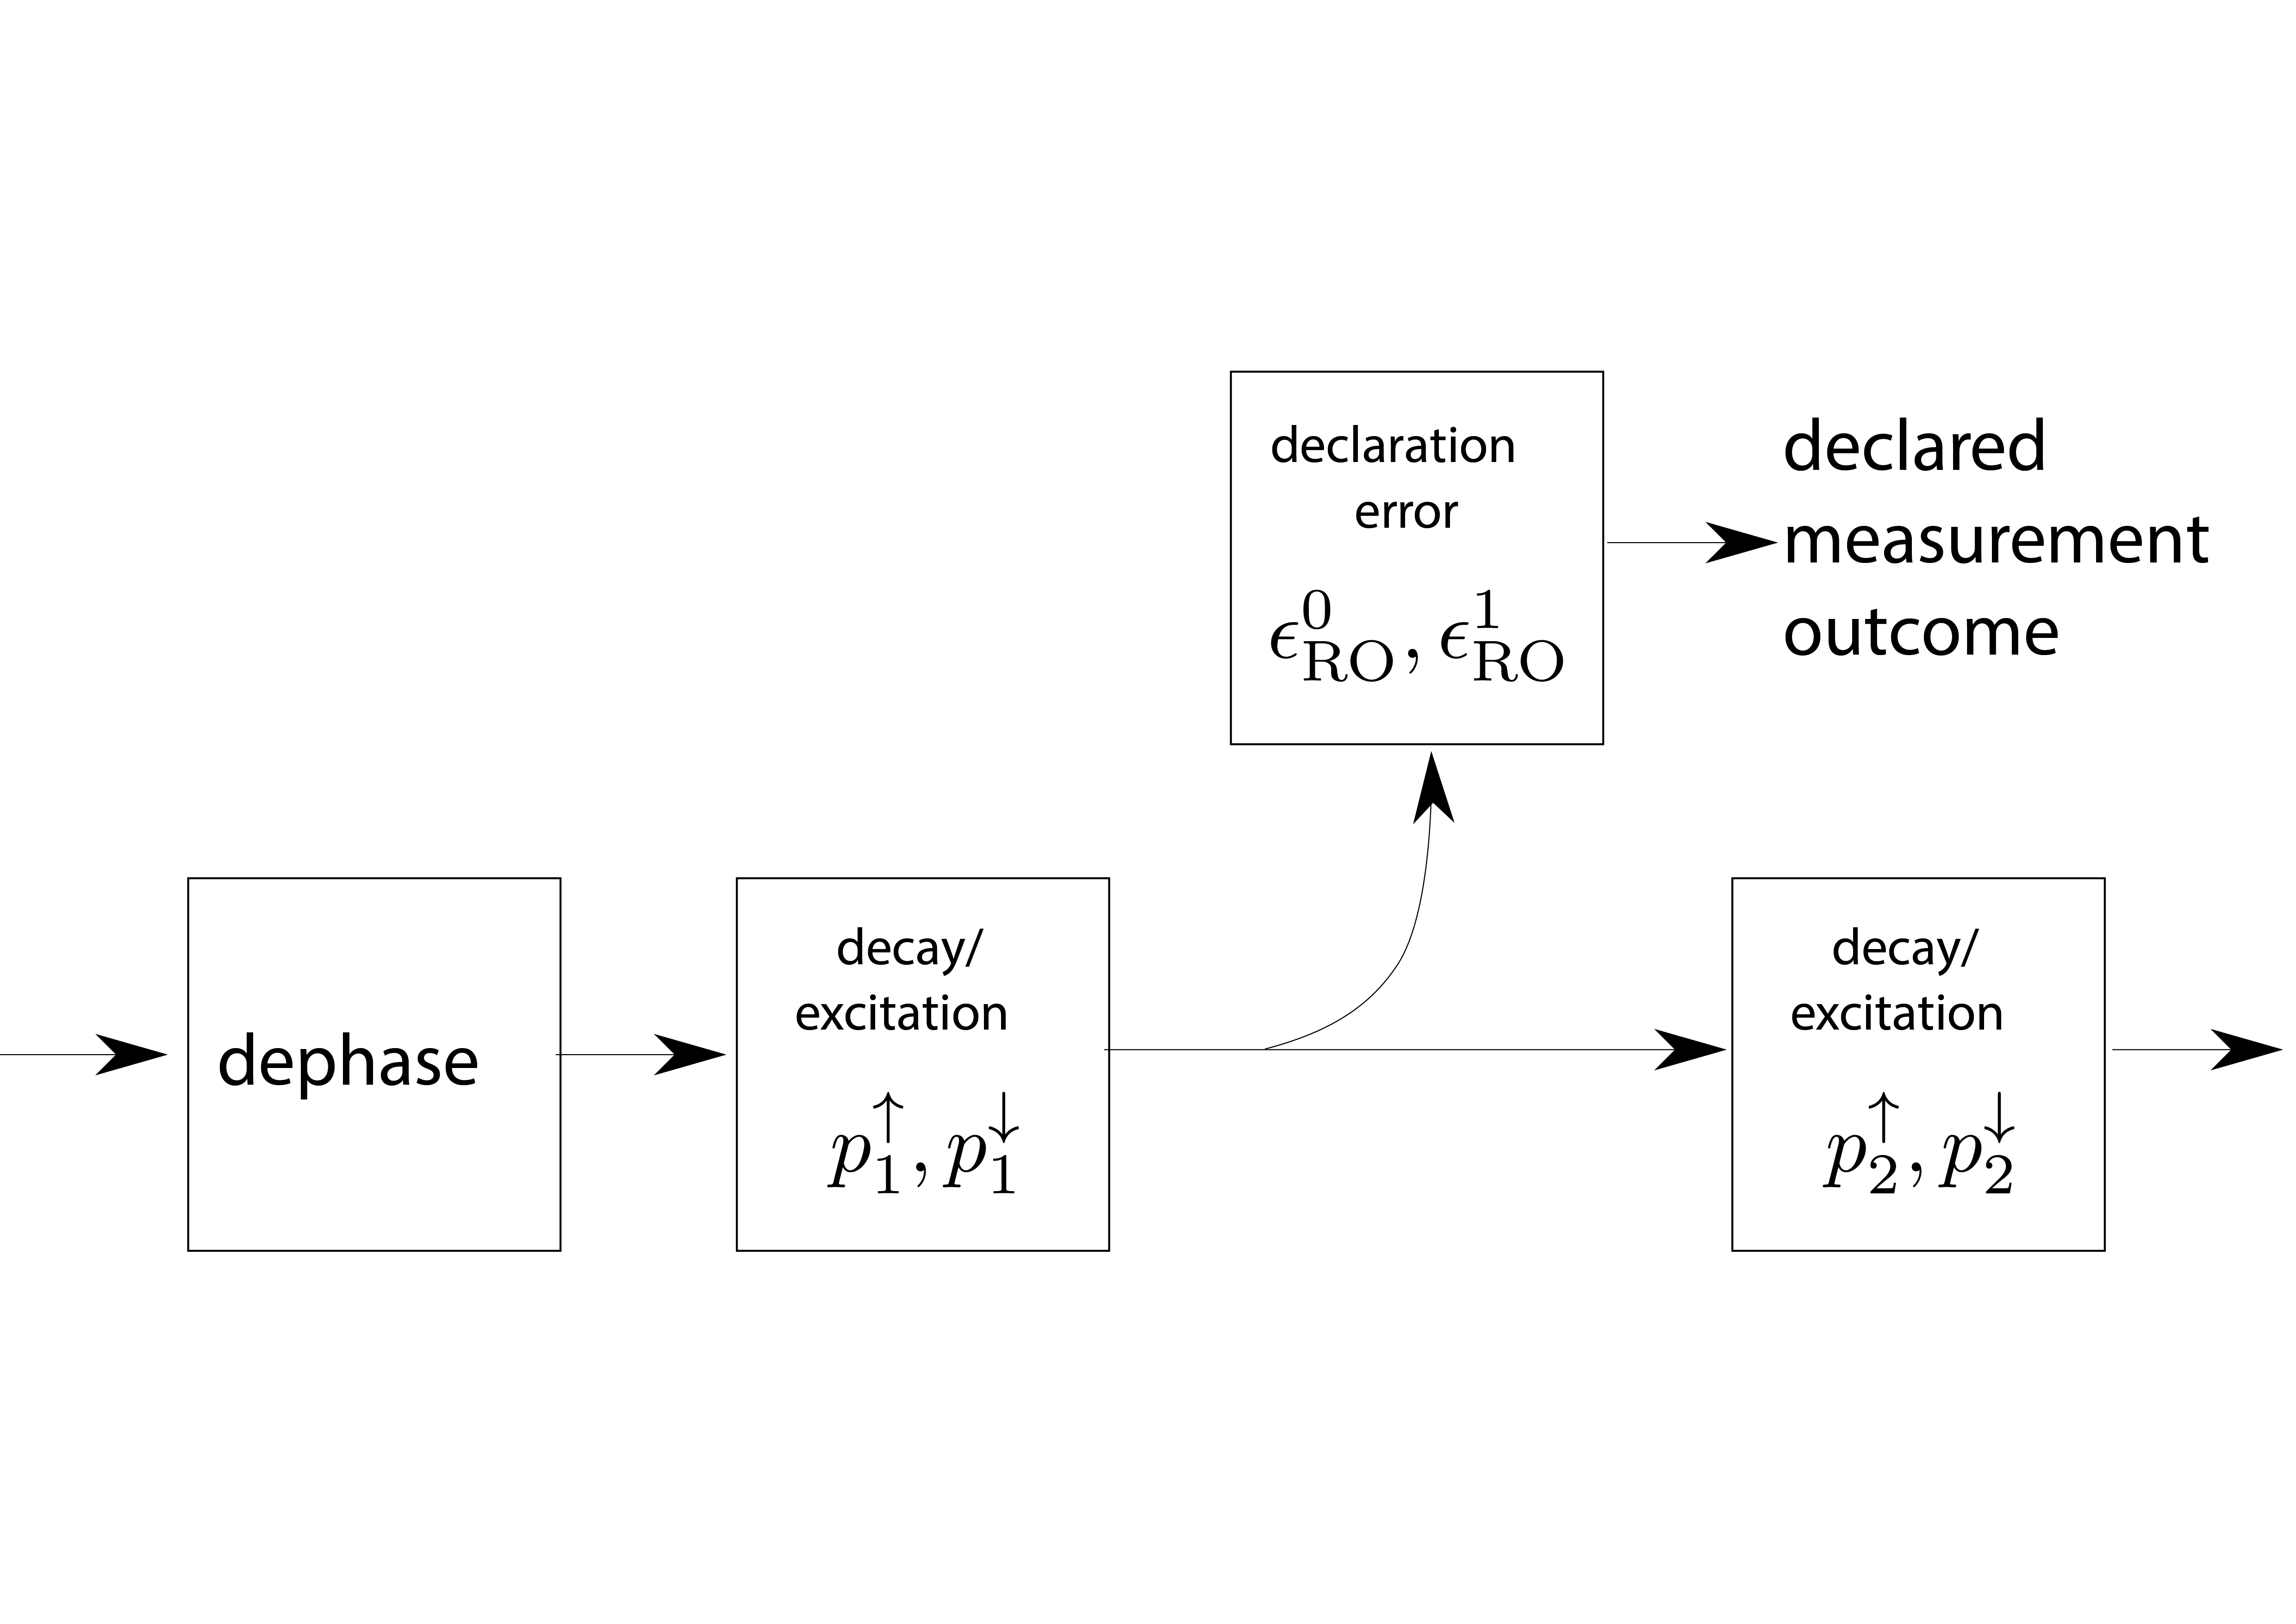
\includegraphics[width=0.5\textwidth]{figures/measure_model.png}
\caption{\label{fig:org7d44807}
The model for measurements consists of a dephasing of the qubit followed by a period of decay and excitation with probability \(p_{\uparrow / \downarrow}^{(1)}\). At this point, the qubit state is sampled. The sampling result is subject to a declaration error \(\epsilon_{RO}\), and the qubit state is subject to further decay or excitation with probabilities \(p_{\uparrow / \downarrow}^{(2)}\) before the end of the measurement block}
\end{figure}

The initial dephasing step in the measurement model (Fig. \ref{fig:org7d44807}) occurs due to the \hyperref[sec:org0f14c52]{photon decay} effect.

"We find that the readout errors \(\epsilon_{RO}^{|i\rangle}\) are almost independent of the qubit state \(|i\rangle\), and so we describe them with a single readout error parameter \(\epsilon_{RO}\)".
The outcome-independent declaration error of \(\epsilon_{RO} = \epsilon_{RO}^{1} = \epsilon_{RO}^{0} = 0.15 \%\) is extracted from experiments. 

They ignore effects leading to measurement-induced mixing and non-linearity of the readout resonator, as well as residual photon numbers.

\item Photon decay
\label{sec:org0f14c52}
In the presence of photons in a readout resonator, the coupled qubit is affected suffering a \(p_{\phi, photon}\) dephasing.
This dephasing is present whenever the coupled qubit is brought into superposition before the readout resonator has returned to the vacuum state following the last measurement.
This dephasing is then implemented via the same Pauli transfer matrix as \(R_{\Lambda_{T_{\phi}}}\).

\item Flux Noise
\label{sec:org3d4effb}

During a quantum algorithm, "transmons are repeatedly moved in frequency away from their sweetspot using flux pulses, either to implement a C-Z gate or to avoid one. Away from the sweetspot, transmons become first-order sensitive to flux noise, which causes an additional random phase shift."

"As this noise typically has a \(1/f\) power spectrum, the largest contribution comes from low-frequency components that are essentially static for a single run, but fluctuating between different runs."
"Shifting the transmon from its sweetspot \(f_{q,max}\) to a lower frequency \(f_q (t)\) makes it first-order sensitive to flux noise".

"In our simulation, we approximate the effect of this noise through ensemble averaging, with quasi-static phase error added to a transmon whenever it is flux pulsed."

As one could see in the figures 4 and 5 from the Supplemental information, a little over-rotation  caused by inaccurate calibration of the flux pulse in a single- or two-qubit gate translates in a huge increase of the \(\epsilon_L\).
\end{itemize}


\item Effects not taking into account
\label{sec:org3cd2a63}

They use a simple model for the CZ errors.
They neglect leakage (previous experiments have reduced leakage probability per CZ to \(\approx\) 0.3\%).
Of course this simplification is also in \textbf{quantumsim}.
\end{itemize}

\subsection*{Error Framework}
\label{sec:org18eefe8}
\begin{figure}[htbp]
\centering
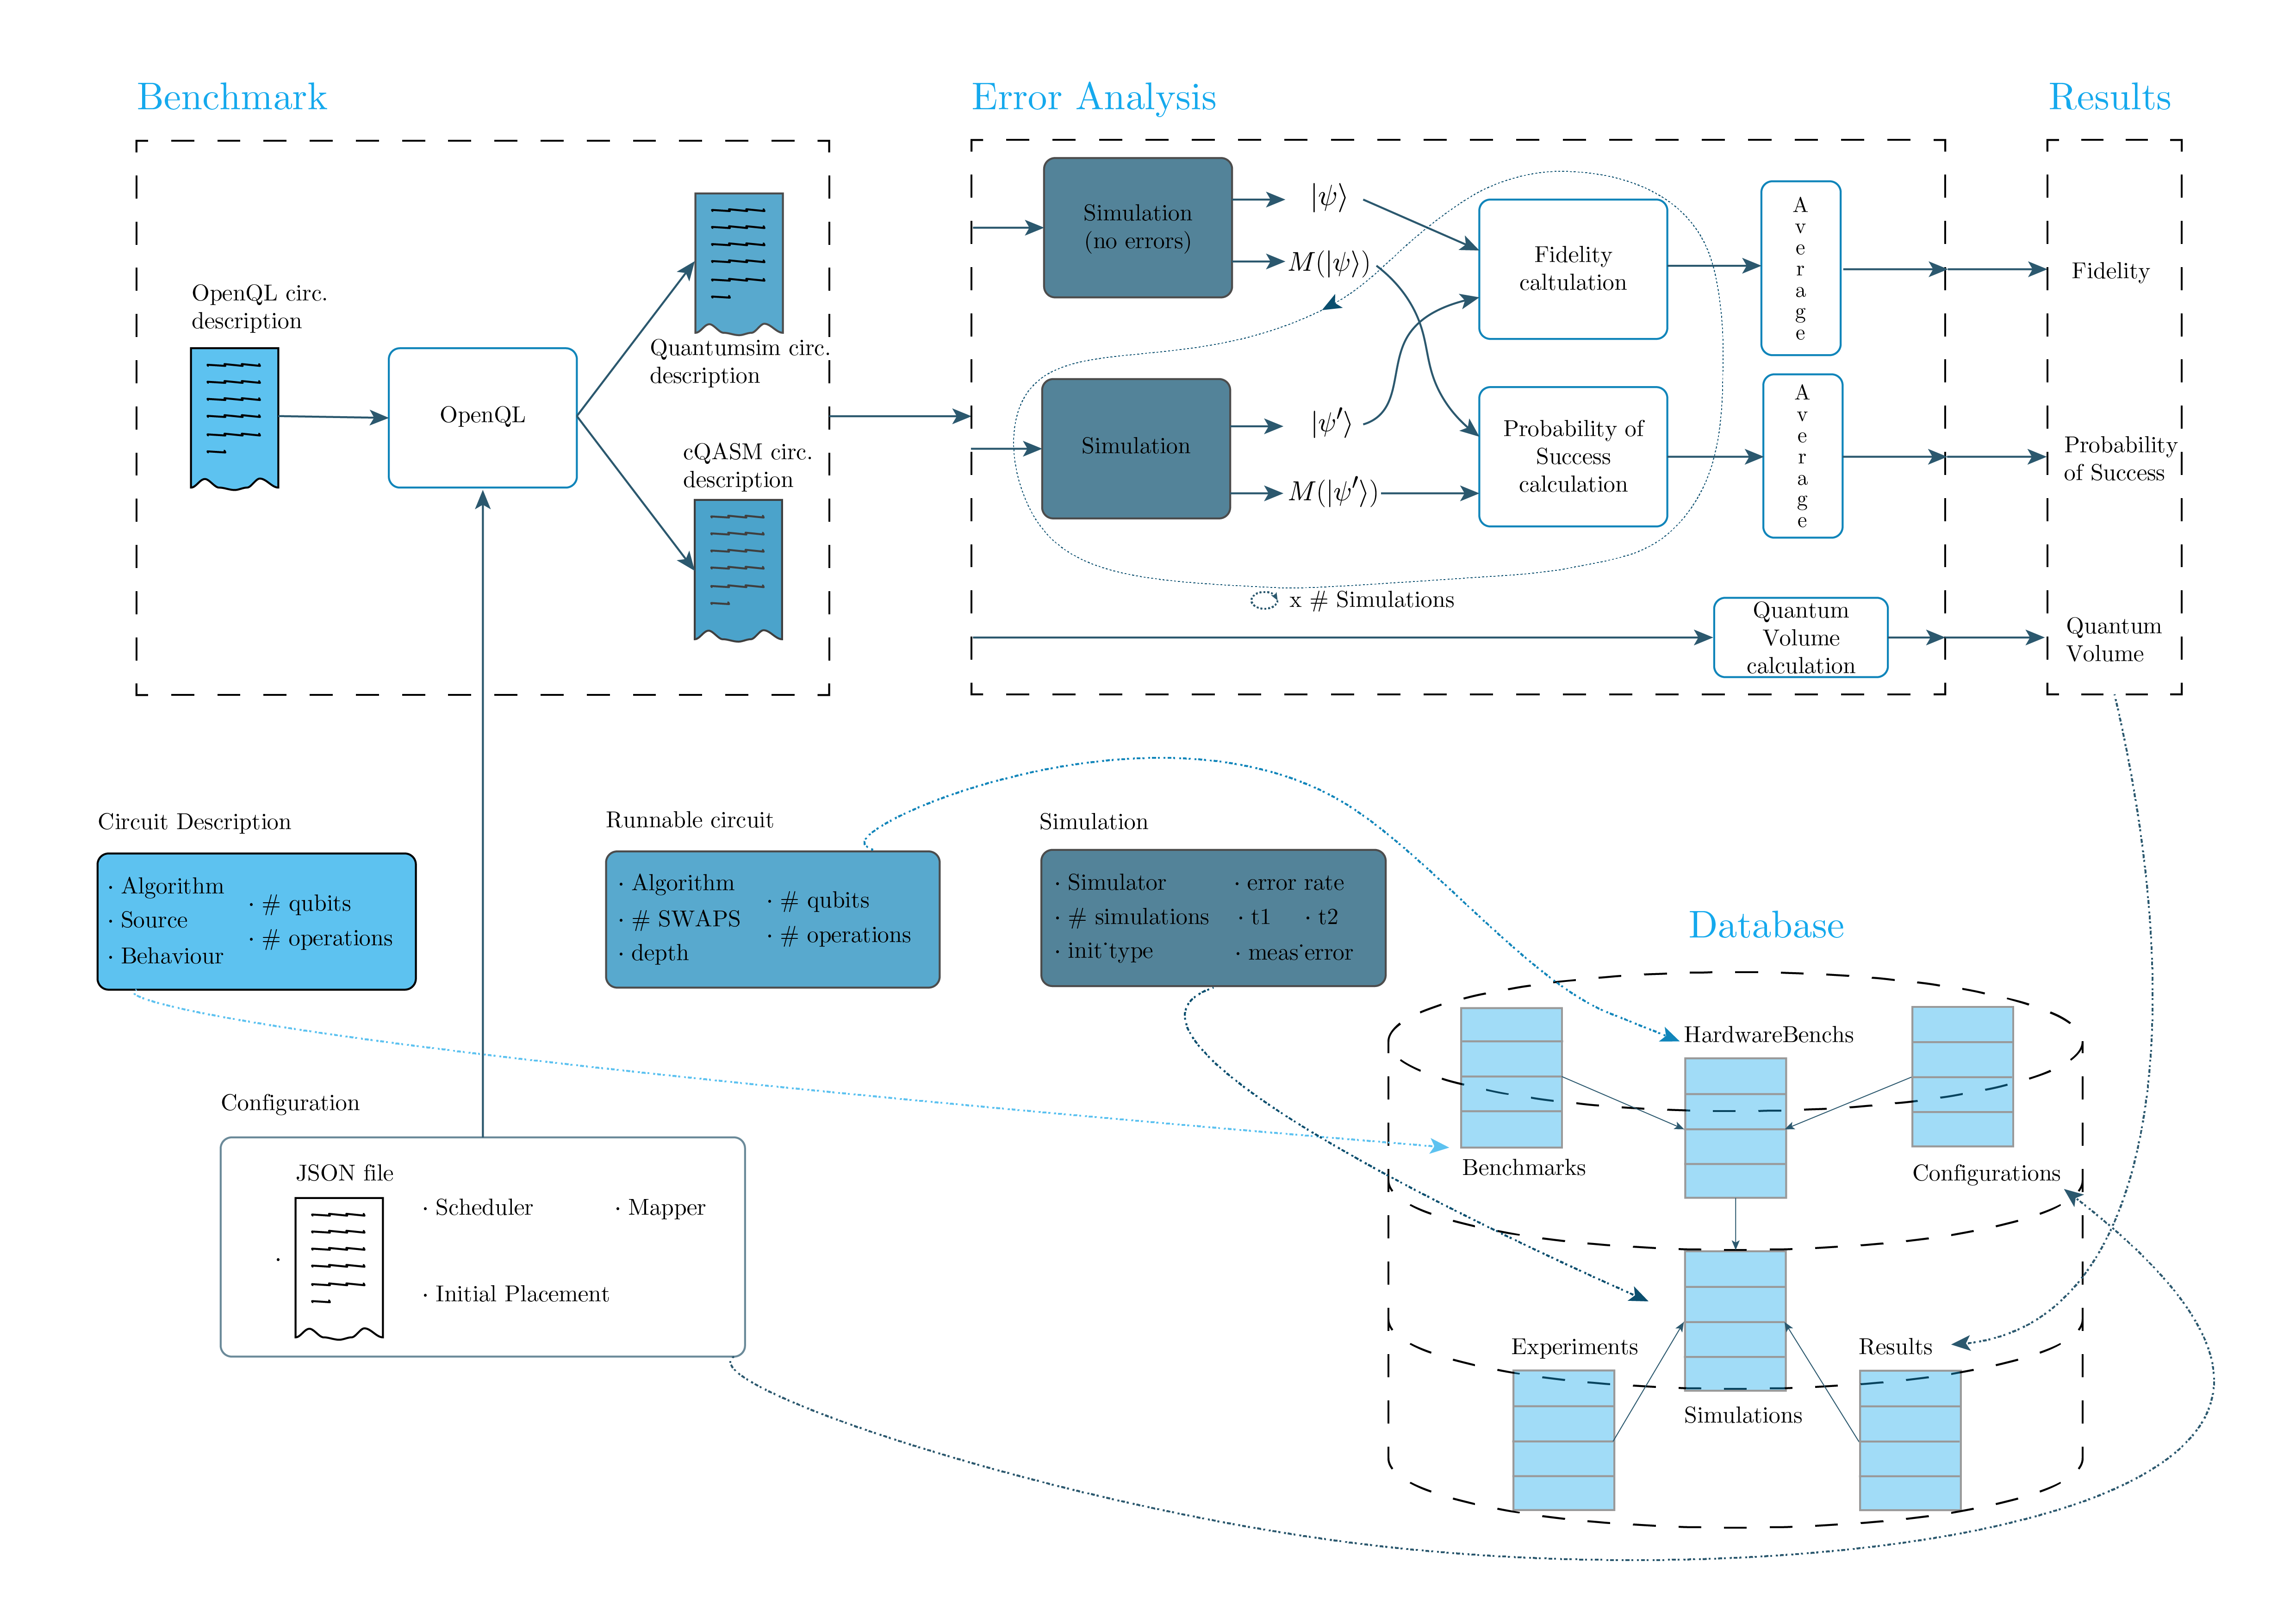
\includegraphics[width=\textwidth]{figures/error_framework_diagram.png}
\caption{\label{fig:orgda36db6}
Error Framework}
\end{figure}

\begin{itemize}
\item Benchmark Object
\label{sec:orga0342ad}

\begin{figure}[htbp]
\centering
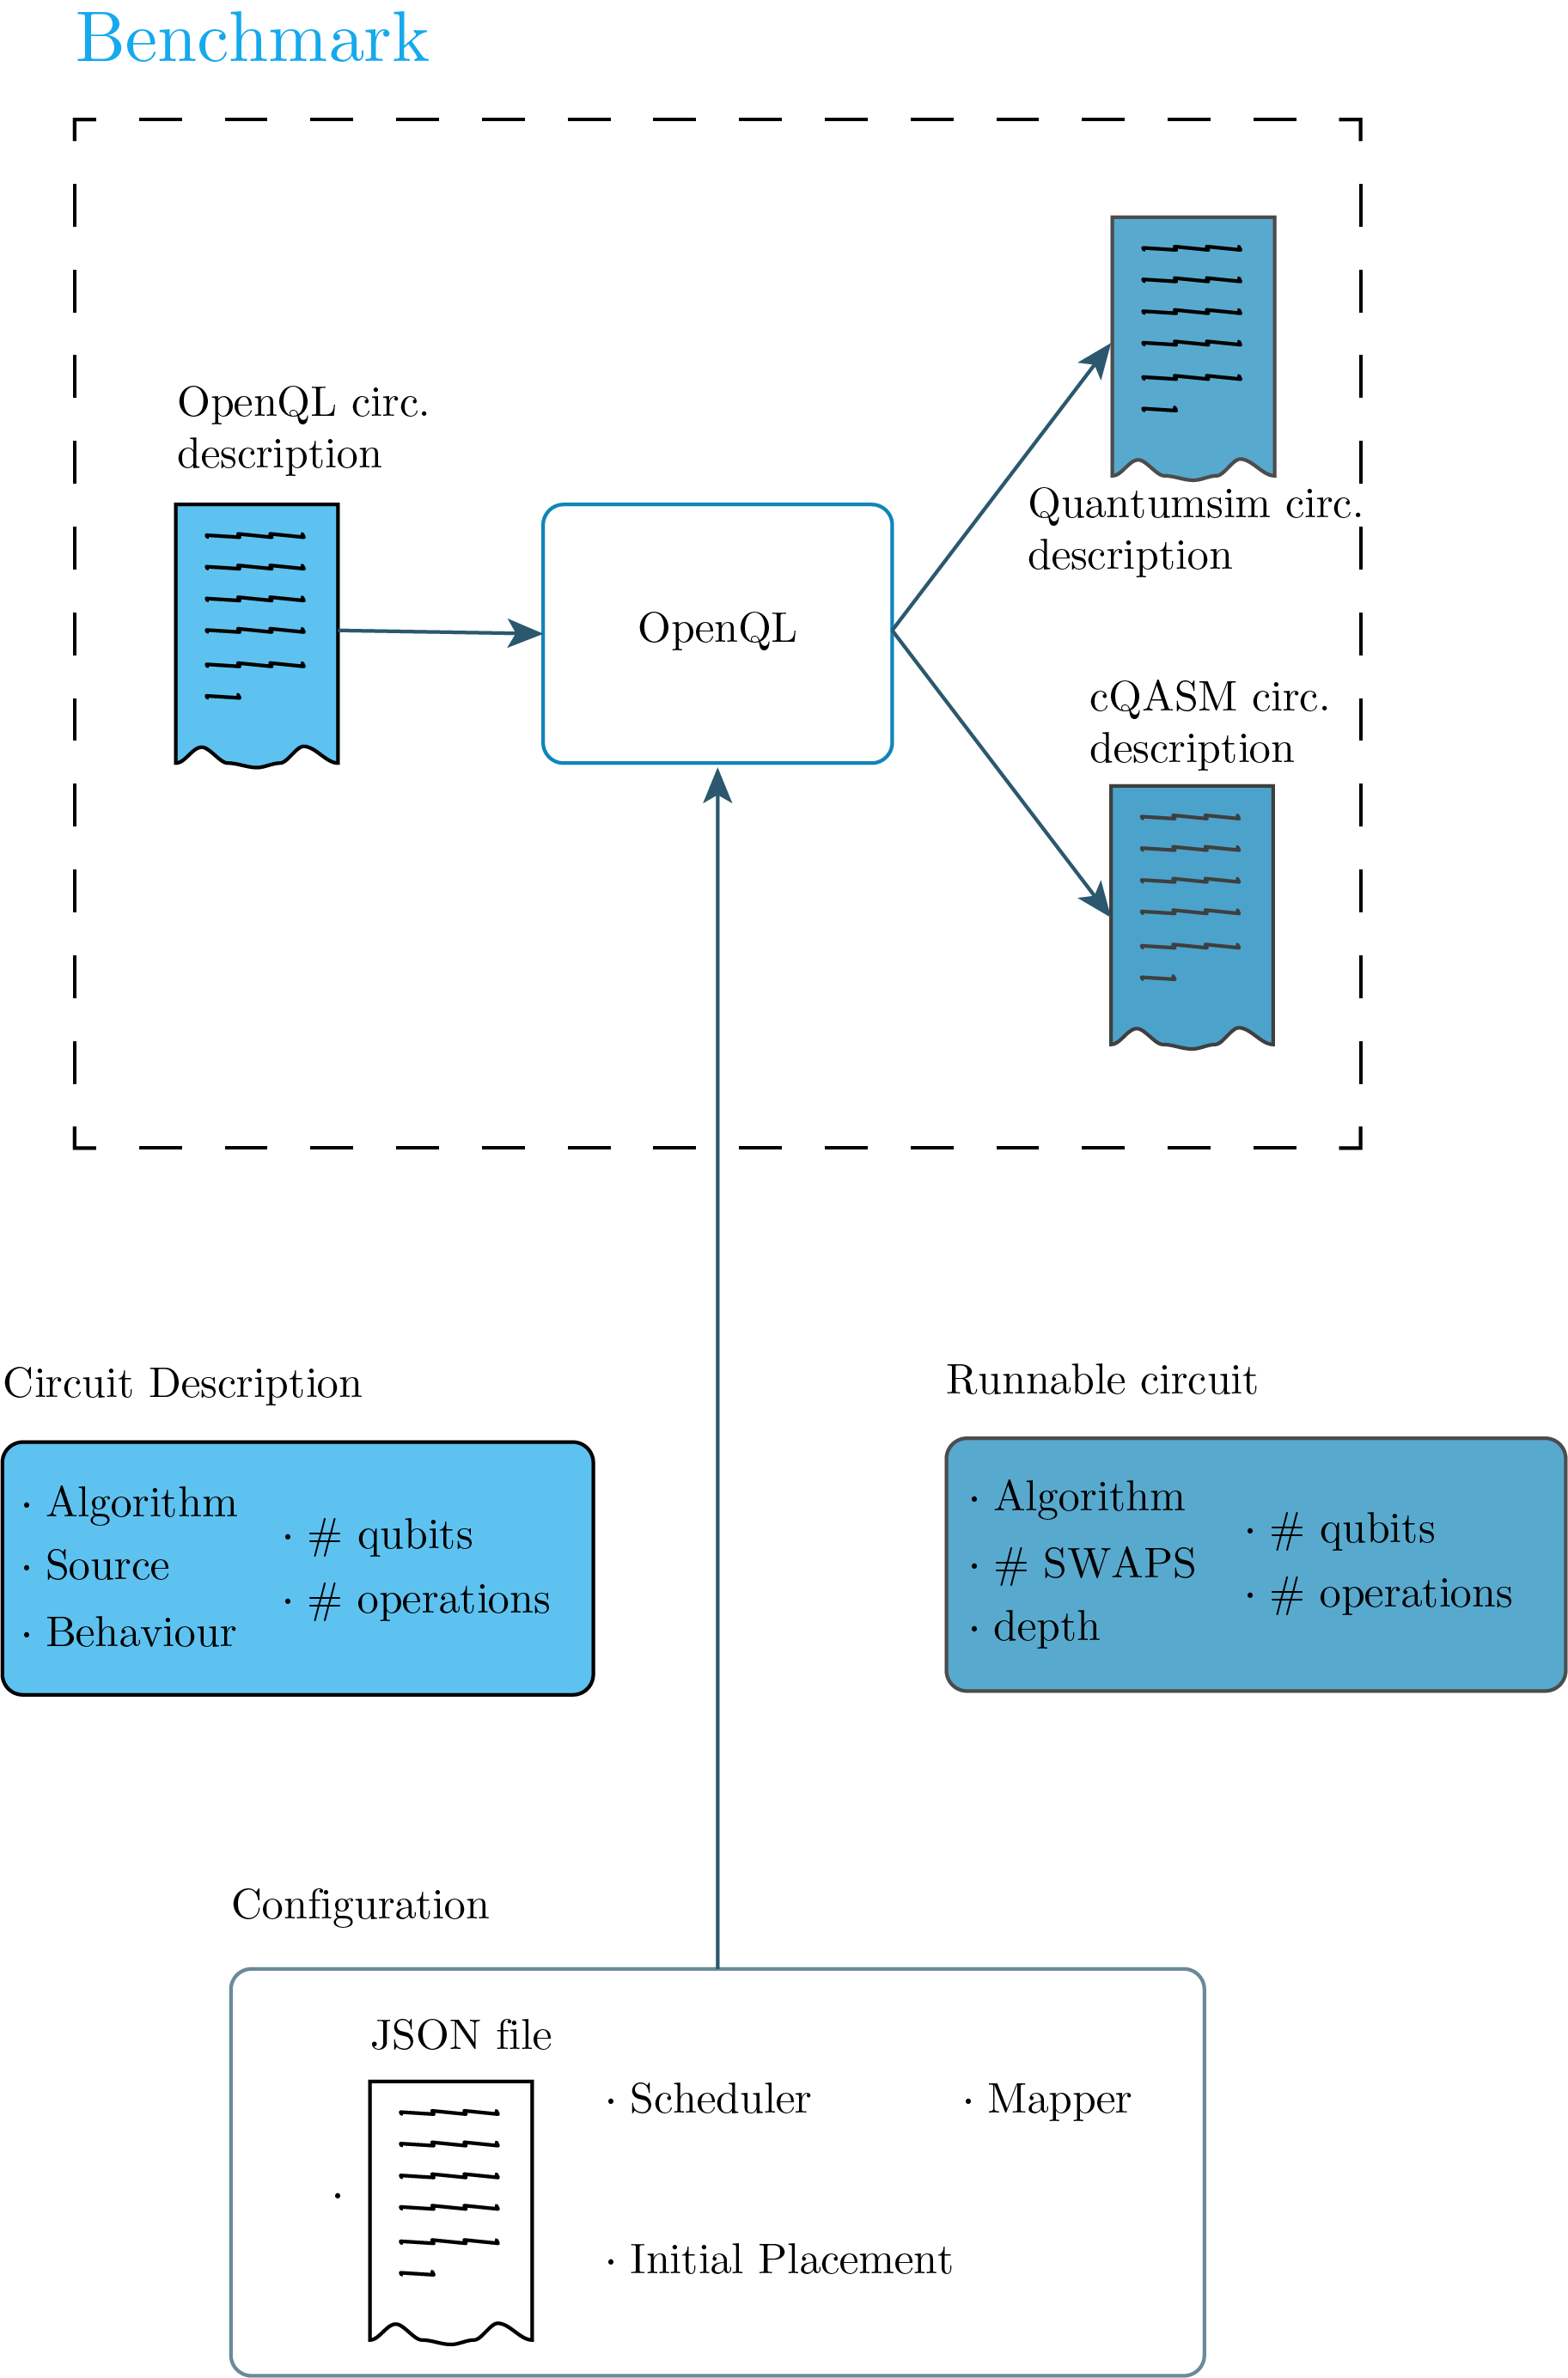
\includegraphics[width=.5\textwidth]{figures/benchmark_object.png}
\caption{\label{fig:org4bafacb}
Benchmark Object \ldots{}}
\end{figure}

\item Mapping Analysis Object
\label{sec:orgd83d6a8}

\begin{figure}[htbp]
\centering
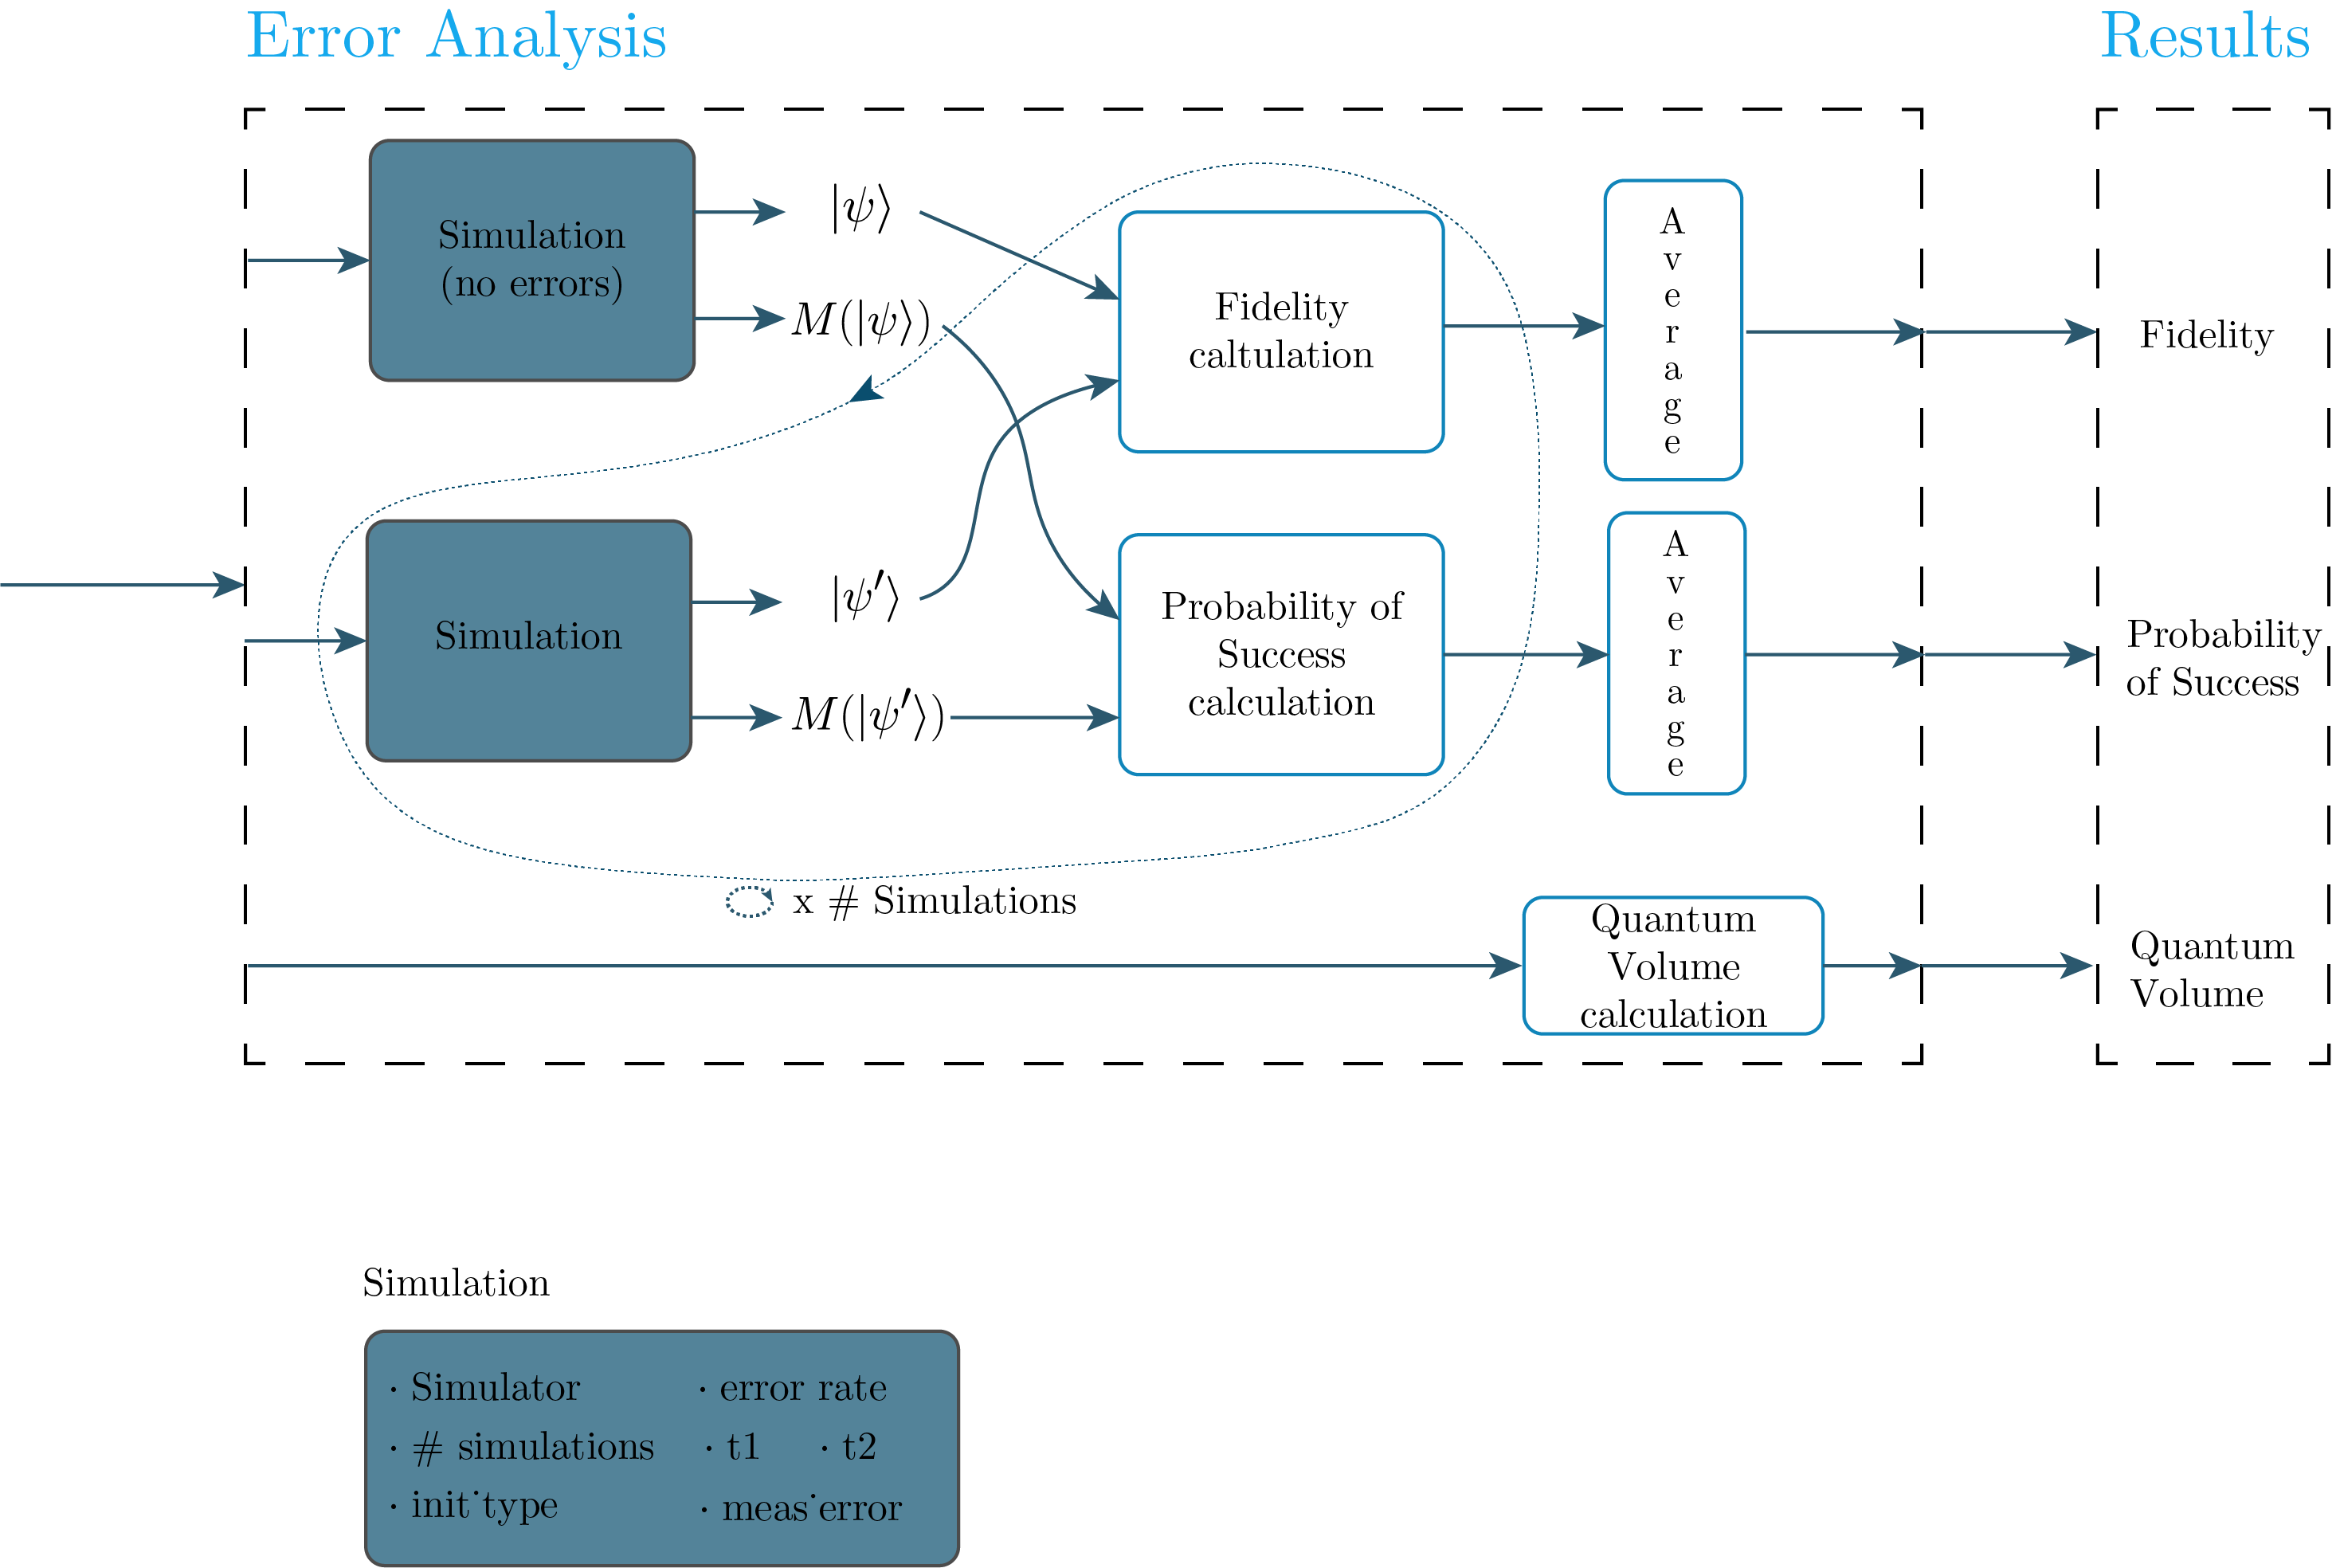
\includegraphics[width=.75\textwidth]{figures/error_analysis.png}
\caption{\label{fig:org30a0fad}
Mapping Analysis Object \ldots{}}
\end{figure}

\item Database
\label{sec:org12cb485}

\begin{figure}[htbp]
\centering
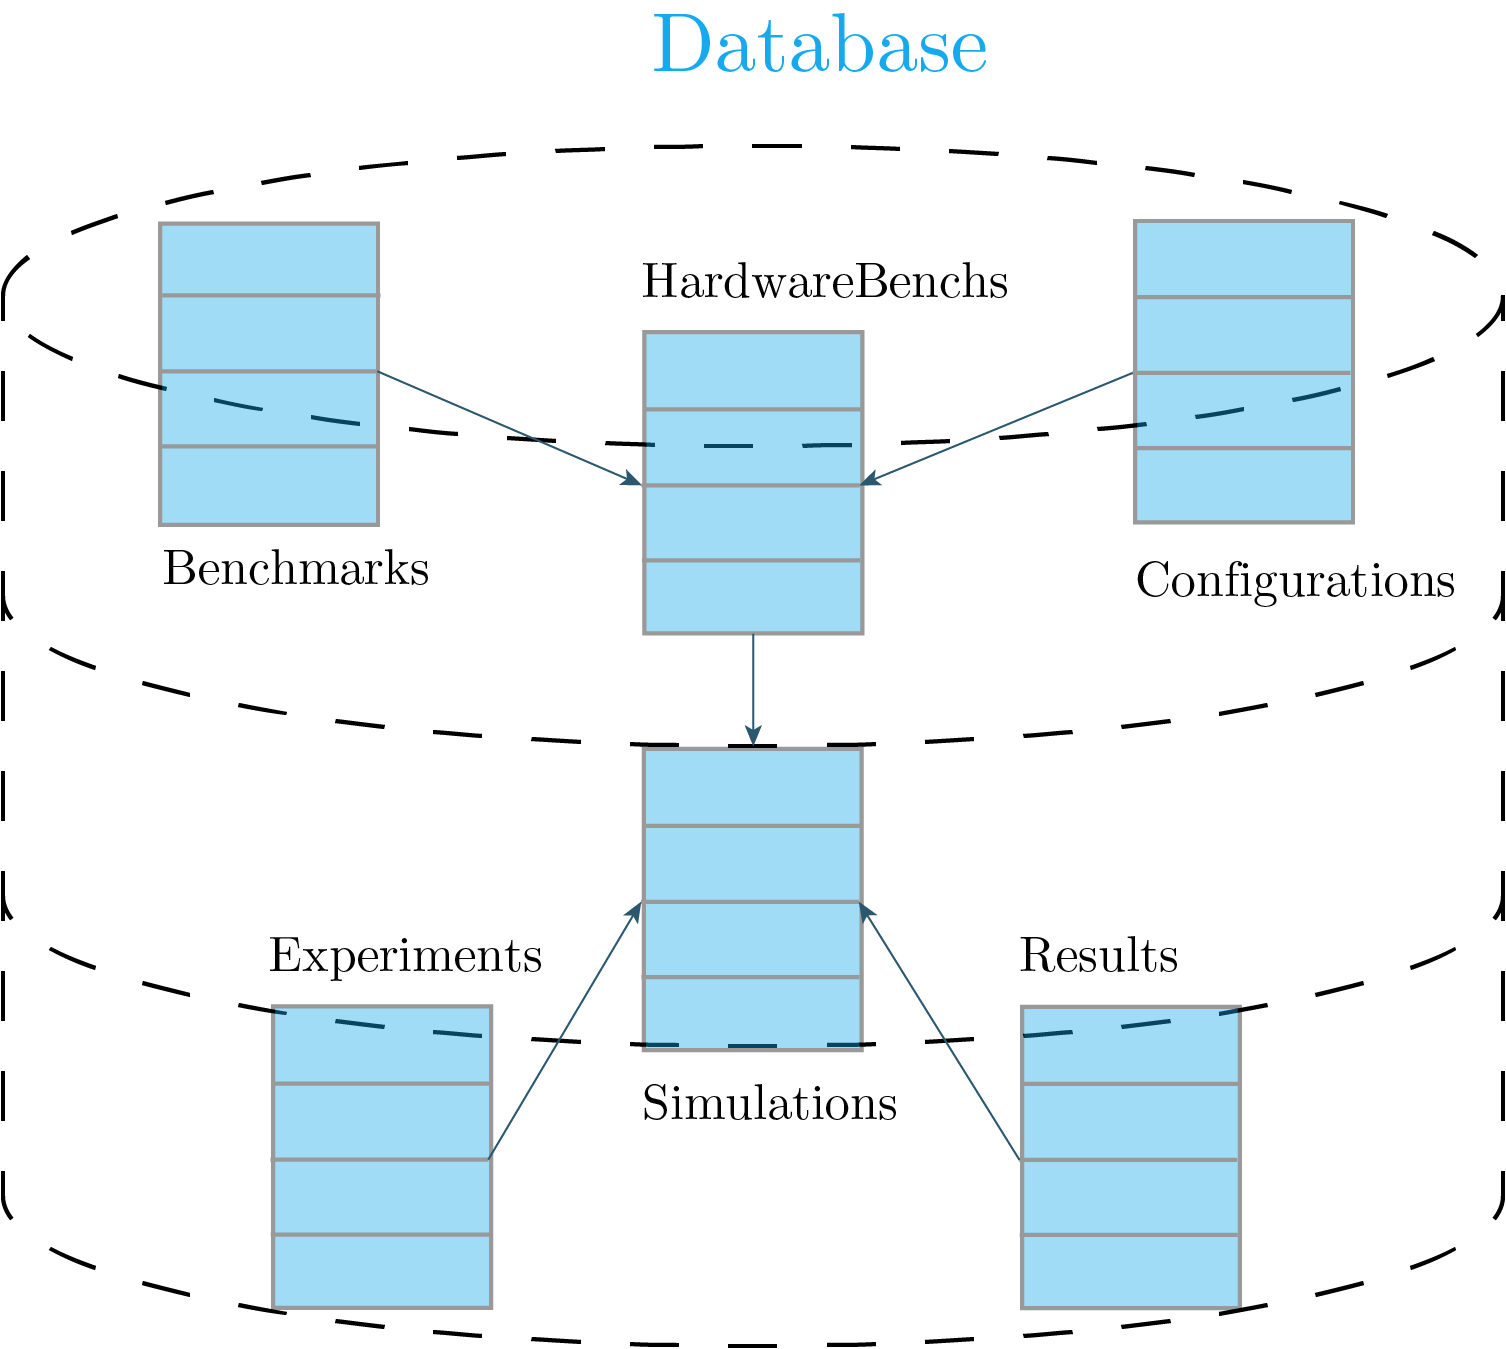
\includegraphics[width=.5\textwidth]{figures/database_scheme_detail.png}
\caption{\label{fig:org23d51a4}
Database tables}
\end{figure}

\begin{figure}[htbp]
\centering
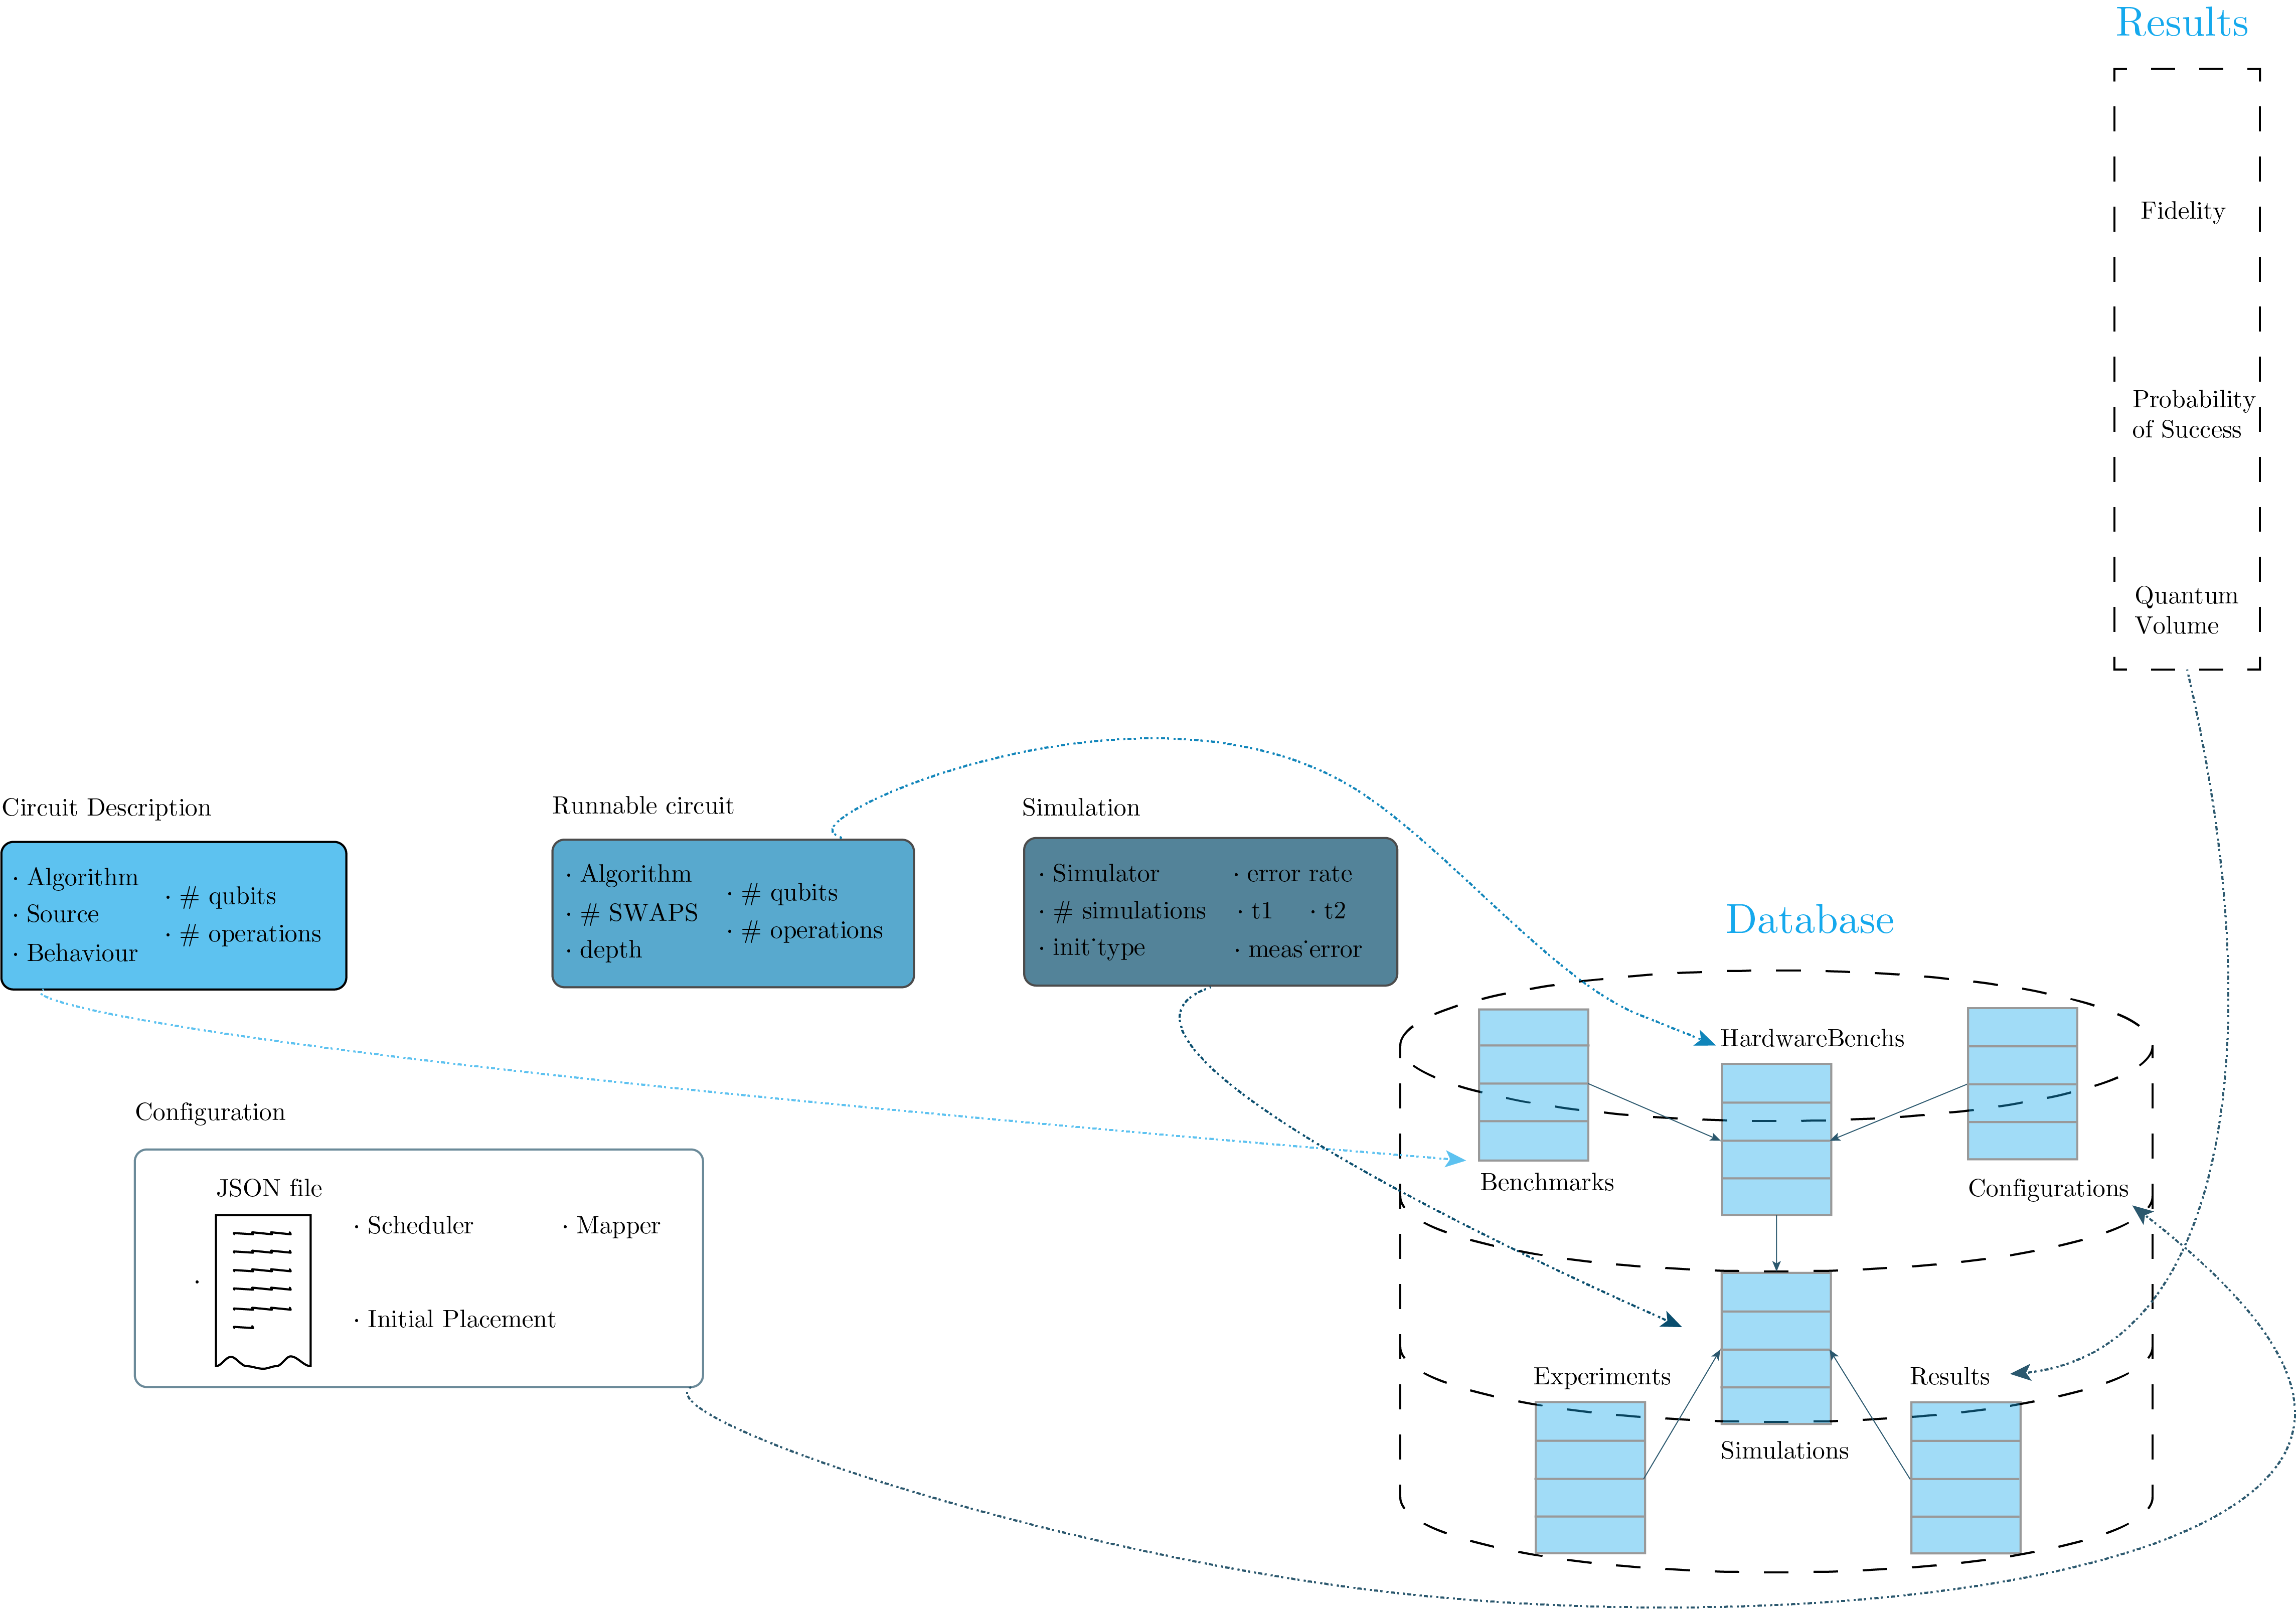
\includegraphics[width=\textwidth]{figures/database_scheme_general.png}
\caption{\label{fig:org244ef32}
Database tables information}
\end{figure}
\end{itemize}
